%===============================================================================
% LaTeX sjabloon voor de bachelorproef toegepaste informatica aan HOGENT
% Meer info op https://github.com/HoGentTIN/bachproef-latex-sjabloon
%===============================================================================

\documentclass{bachproef-tin}

\usepackage{hogent-thesis-titlepage} % Titelpagina conform aan HOGENT huisstijl

\usepackage{biblatex}
\addbibresource{bachproef-tin.bib}

%%---------- Documenteigenschappen ---------------------------------------------
% TODO: Vul dit aan met je eigen info:

% De titel van het rapport/bachelorproef
\title{Het bepalen van een optimale opstelling voor de registratie van een verplaatsing van locatie binnen een gebouw}

% Je eigen naam
\author{Cedric Delaruelle}

% De naam van je promotor (lector van de opleiding)
\promotor{Johan Van Schoor}

% De naam van je co-promotor. Als je promotor ook je opdrachtgever is en je
% dus ook inhoudelijk begeleidt (en enkel dan!), mag je dit leeg laten.
\copromotor{Pieter Suanet}

% Indien je bachelorproef in opdracht van/in samenwerking met een bedrijf of
% externe organisatie geschreven is, geef je hier de naam. Zoniet laat je dit
% zoals het is.
\instelling{Aucxis}

% Academiejaar
\academiejaar{2021-2022}

% Examenperiode
%  - 1e semester = 1e examenperiode => 1
%  - 2e semester = 2e examenperiode => 2
%  - tweede zit  = 3e examenperiode => 3
\examenperiode{2}

%===============================================================================
% Inhoud document
%===============================================================================

\begin{document}

%---------- Taalselectie -------------------------------------------------------
% Als je je bachelorproef in het Engels schrijft, haal dan onderstaande regel
% uit commentaar. Let op: de tekst op de voorkaft blijft in het Nederlands, en
% dat is ook de bedoeling!

%\selectlanguage{english}

%---------- Titelblad ----------------------------------------------------------
\inserttitlepage

%---------- Samenvatting, voorwoord --------------------------------------------
\usechapterimagefalse
%%=============================================================================
%% Voorwoord
%%=============================================================================

\chapter*{\IfLanguageName{dutch}{Woord vooraf}{Preface}}
\label{ch:voorwoord}

%% TODO:
%% Het voorwoord is het enige deel van de bachelorproef waar je vanuit je
%% eigen standpunt (``ik-vorm'') mag schrijven. Je kan hier bv. motiveren
%% waarom jij het onderwerp wil bespreken.
%% Vergeet ook niet te bedanken wie je geholpen/gesteund/... heeft


%%=============================================================================
%% Samenvatting
%%=============================================================================

% TODO: De "abstract" of samenvatting is een kernachtige (~ 1 blz. voor een
% thesis) synthese van het document.
%
% Deze aspecten moeten zeker aan bod komen:
% - Context: waarom is dit werk belangrijk?
% - Nood: waarom moest dit onderzocht worden?
% - Taak: wat heb je precies gedaan?
% - Object: wat staat in dit document geschreven?
% - Resultaat: wat was het resultaat?
% - Conclusie: wat is/zijn de belangrijkste conclusie(s)?
% - Perspectief: blijven er nog vragen open die in de toekomst nog kunnen
%    onderzocht worden? Wat is een mogelijk vervolg voor jouw onderzoek?
%
% LET OP! Een samenvatting is GEEN voorwoord!

%%---------- Nederlandse samenvatting -----------------------------------------
%
% TODO: Als je je bachelorproef in het Engels schrijft, moet je eerst een
% Nederlandse samenvatting invoegen. Haal daarvoor onderstaande code uit
% commentaar.
% Wie zijn bachelorproef in het Nederlands schrijft, kan dit negeren, de inhoud
% wordt niet in het document ingevoegd.

\IfLanguageName{english}{%
\selectlanguage{dutch}
\chapter*{Samenvatting}
\lipsum[1-4]
\selectlanguage{english}
}{}

%%---------- Samenvatting -----------------------------------------------------
% De samenvatting in de hoofdtaal van het document

\chapter*{\IfLanguageName{dutch}{Samenvatting}{Abstract}}

\lipsum[1-4]


%---------- Inhoudstafel -------------------------------------------------------
\pagestyle{empty} % Geen hoofding
\tableofcontents  % Voeg de inhoudstafel toe
\cleardoublepage  % Zorg dat volgende hoofstuk op een oneven pagina begint
\pagestyle{fancy} % Zet hoofding opnieuw aan

%---------- Lijst figuren, afkortingen, ... ------------------------------------

% Indien gewenst kan je hier een lijst van figuren/tabellen opgeven. Geef in
% dat geval je figuren/tabellen altijd een korte beschrijving:
%
%  \caption[korte beschrijving]{uitgebreide beschrijving}
%
% De korte beschrijving wordt gebruikt voor deze lijst, de uitgebreide staat bij
% de figuur of tabel zelf.

\listoffigures
\listoftables
\lstlistoflistings

% Als je een lijst van afkortingen of termen wil toevoegen, dan hoort die
% hier thuis. Gebruik bijvoorbeeld de ``glossaries'' package.
% https://www.overleaf.com/learn/latex/Glossaries

%---------- Kern ---------------------------------------------------------------

% De eerste hoofdstukken van een bachelorproef zijn meestal een inleiding op
% het onderwerp, literatuurstudie en verantwoording methodologie.
% Aarzel niet om een meer beschrijvende titel aan deze hoofstukken te geven of
% om bijvoorbeeld de inleiding en/of stand van zaken over meerdere hoofdstukken
% te verspreiden!

%%=============================================================================
%% Inleiding
%%=============================================================================

\chapter{Inleiding}
\label{ch:inleiding}

\section{Probleemstelling}
\label{sec:probleemstelling}

Momenteel is Aucxis, de opdrachtgever en partner voor dit onderzoek, bezig met het uitwerken en ontwikkelen van hun Polaris platform. Het voornaamste doel van dit platform is het kunnen volgen van voorwerpen binnen en buiten bedrijven. Dit aan de hand van verschillende technologieën, voornamelijk RFID en BLE binnen het bedrijf, en GPS daarbuiten. 
Het concept van dit platform is dat er logische locaties bestaan (zoals warenhuis 1 of keuken), waar de voorwerpen zich bevinden. Voor een goede werking van dit systeem is het duidelijk nodig dat uit de data bekomen uit de hardware kan afgeleid worden op welke logische locatie een voorwerp zich bevind en wanneer het zich verplaatst tussen locaties. Dit is geen normaal softwareprobleem want logischerwijs zal de manier waarop de hardware staat opgesteld een grote invloed hebben op de nauwkeurigheid en correctheid van deze lokalisaties en verplaatsingen. Hierdoor is het van groot belang voor de correcte werking van dit platform dat er een goede opstelling wordt gekozen. Om dit te kunnen doen is er een onderzoek nodig naar wat deze optimale opstelling zou kunnen zijn. Dit is ook de reden dat dit onderzoek in het leven is geroepen.

\section{Wie is Aucxis}
\label{sec:wie-is-aucxis}
Aucxis is een bedrijf gevestigd te Stekene, welke actief is sinds 1983. Bij oprichting was het een bedrijf dat zich toespitste op het ontwikkelen van eenderzijds de bewaring (Procescontrole), en anderzijds de veilinginfrastructuur (E-trade) voor groenten en fruit. Het werd hier vrij snel een toonaangevend bedrijf en werd wereldleider tegen 2000. Later, in 2007 richtten ze een 3e businessunit op, namelijk de RFID divisie, welke zich focust op het onderzoek naar en ontwikkeling van RFID toepassingen. Vandaag is het nog steeds een toonaangevend bedrijf met in-house oplossingen voor allerhande toepassingen binnen deze sectoren en zijn ze nog steeds actief bezig aan de optimalisering en uitbreiding hiervan. Recentelijk zijn ze ook geïnteresseerd geworden in het uitbreiden van hun praktijken naar BLE toepassingen.\autocite{Aucxis2020}

\section{Onderzoeksvraag}
\label{sec:onderzoeksvraag}

Zoals duidelijk is geworden in de probleemstelling is er nood aan een onderzoek voor het vinden van een zo optimaal mogelijke opstelling voor het bepalen van de locatie waar een voorwerp zich bevind. Verder is ook de detectie van een verplaatsing belangrijk, dit gebeurt als de locatie van het voorwerp verandert. Met oog op deze probleemstelling luidt de onderzoeksvraag voor deze bachelorproef als volgt:
\begin{center}
	\textbf{Welke hardwareopstelling, bestaande uit RFID of BLE componenten, is optimaal voor de plaats- en verplaatsingsbepaling van een voorwerp binnen een gebouw.}
\end{center}
Deze vraag omvangt goed de essentie van de situatie die dient onderzocht te worden, namelijk de beste opstelling voor het volgen van een voorwerp binnen een gebouw, en dit met RFID of BLE technologie. Binnen de probleemstelling werd echter ook aangegeven dat binnen de scope van Polaris ook gps lokalisatie voor voorwerpen buiten het bedrijf aanwezig was. Locatiebepaling met behulp van gps is echter al goed ingeburgerd, waardoor er voldoende bronnen zijn en dit ook duidelijk en precies is. Door deze reden is er geen nut om dit ook te onderzoeken en wordt dit onderdeel buiten de scope van dit onderzoek gehouden. Plaatsbepalingen binnen zijn echter niet zo optimaal voor gps aangezien de meeste gebouwen/kantoren beschikken over verdiepen (waar er meerdere locaties dezelfde geografische coördinaat hebben), en gps ook een bepaalde onzekerheid heeft op de meting.

\section{Onderzoeksdoelstelling}
\label{sec:onderzoeksdoelstelling}

Het hoofddoel van dit onderzoek is het vergelijken van een aantal opstellingen, met RFID of met BLE, en met verschillende concepten achter hun werking. De verschillende opstellingen met hun theoretische achtergrond volgen verder in dit verslag. Zoals de onderzoeksvraag echter al doet vermoeden is het doel niet louter een vergelijkende studie, aangezien het ook de bedoeling is dat er een optimale opstelling uit de bus komt. 
In praktijk zal er nooit een opstelling zijn die de beste is, aangezien er altijd een afweging zal zijn tussen de nauwkeurigheid en de kostprijs van de opstelling. Ook zullen sommige opstellingen beter zijn in bepaalde situaties dan andere. Wel zal het mogelijk zijn om totaal onpraktische en onnauwkeurige opstellingen uit te branden. De conclusie zal eerder een afweging geven tussen de verschillende opstellingen, maar zal zeker geen louter vergelijkende aard hebben.

\section{Opzet van dit onderzoek}
\label{sec:opzet-bachelorproef}

De rest van dit onderzoek is als volgt opgebouwd:

In Hoofdstuk~\ref{ch:literatuurstudie} wordt een overzicht gegeven van de theoretische achtergrond die nodig is voor het begrijpen van het onderzoek en de rest van dit onderzoek. Het bevat informatie over de werking van de RFID en BLE technologieën, definities van veelvoorkomende begrippen en diverse andere benodigde uitleg.

In Hoofdstuk~\ref{ch:opstellingen} worden de onderzochte opstellingen opgesomd, samen met een theoretische achtergrond. Het is een projectie van de kennis opgedaan tijdens de literatuurstudie op de te onderzoeken opstellingen.

In Hoofdstuk~\ref{ch:methodologie} wordt de methodologie toegelicht en worden de gebruikte onderzoekstechnieken besproken om een antwoord te kunnen formuleren op de onderzoeksvraag.

In Hoofdstuk~\ref{ch:testen} worden de uitgevoerde tests beschreven, de resultaten verwerkt en geconcludeerd.

In Hoofdstuk~\ref{ch:conclusie}, tenslotte, wordt eerst de voornaamste informatie gebundeld, waarna deze gebruikt wordt om een algemene conclusie te gegeven en een antwoord te formuleren op de onderzoeksvraag. Daarna wordt ook een aanzet gegeven voor toekomstig onderzoek binnen dit domein.
%%=============================================================================
%% Literatuurstudie
%%=============================================================================

\chapter{Literatuurstudie}
\label{ch:literatuurstudie}

Dit hoofdstuk zal een overzicht geven van de theoretische achtergrond van de hardware, protocollen, programma's en andere concepten die gebruikt worden bij het gevoerde onderzoek voor het beantwoorden van bovengenoemde onderzoeksvraag.

\section{Definities}
\label{sec:lit-definities}
Deze sectie zal enkele belangrijke begrippen introduceren die belangrijk zullen zijn bij het verdere lezen van dit hoofdstuk en de rest van het document.

\subsubsection{RSSI}
De RSSI, of voluit Received Signal Strength Indicator, is een maat voor de signaalsterkte die een ontvanger ontvangt van bijhorende zender. Ze wordt typisch gebruikt als het over radio-/elektromagnetische golven gaat.\autocite{Admin2022} Ze wordt uitgedrukt in dBm (Decibel per milliwatt).\autocite{Tseard2016} Het is een zeer kleine en logaritmische maat, de waarden in dit document zullen in de grootteorde -10 dBm liggen.

\subsubsection{IoT}
IoT, of voluit Internet Of Things, is een systeem van samenwerkende devices die met elkaar verbonden zijn via het internet, en zo, zonder menselijke tussenkomst, taken uitvoeren. Elk device is geïdentificeerd door een unieke identifier, of UID. Een device in deze context is alles wat met het internet kan verbonden zijn.\autocite{Gillis2022}

\subsubsection{MQTT}
MQTT, of voluit Message Queuing Telemetry Transport, is een protocol voor het versturen van berichten gemaakt door IoT devices over het internet. Belangrijke voordelen van het protocol zijn dat het licht en efficiënt is, en gemakkelijk schaalbaar naar grote hoeveelheden devices.\autocite{MQTT2022}

\subsubsection{FSPL}
FSPL, of voluit Free Space Path Loss, is het theoretische verlies in signaalsterkte over een bepaalde afstand in open ruimte. Deze kan berekend worden, gegeven de afstand tussen de 2 antennes (d), de frequentie van de EM golf (f), en de gain op de zendende en ontvangende antenne (Gz en Go respectievelijk). Ze wordt berekend via onderstaande formule: 
\[FSPL = 20\log_{10}(d) + 20\log_{10}(f) + 20\log_{10}(\frac{4\pi}{c}) - G_z - G_o \]
\autocite{Pasternack2020}

In deze formule staat \(c\) voor de lichtsnelheid \(\approx3x10^5 \frac{m}{s}\)
\autocite{SOL2022}

\subsubsection{Trilateratie}
Trilateratie is de berekening voor de bepaling van de coördinaten van een punt uit 2 geweten punten, en de afstanden van die punten tot het te berekenen punt. Uit deze berekening blijven 2 punten over, 1 boven en 1 onder de lijn tussen de 2 geweten punten. Hiervan is er steeds 1 mogelijk en 1 onmogelijk, dit onmogelijke punt kan hierdoor logisch uitgebrand worden. De formules voor berekening zijn als volgt:
 \[x = \frac{d_1^2 - d_2^2 + (x_2 - x_1)}{2(x_2 - x_1)} + x_1\]
 \[y = \sqrt{d_1^2 - x^2} \pm y_1\]
 Met \((x,  y)\) de coördinaten van het onbekende punt,  \((x_1, y_1)\) en \((x_2, y_1)\) de coördinaten van de geweten punten en \(d_1\) en \(d_2\) de bekende afstanden.
 \autocite{TRM2022}

\section{Hardware}
\label{sec:lit-hardware}
Deze sectie zal de gebruikte hardwaretechnologieën toelichten, deze zijn RFID en BLE.

\subsection{RFID}
\label{subsec:lit-rfid}
RFID, of voluit Radio Frequency IDentification, is een draadloos communicatie systeem welke gebruik maakt van elektromagnetische golven\footnote{Verder in dit document worden deze afgekort als EM golven}. Een typische RFID opstelling bestaat uit 3 delen, nl. een zender/ontvanger combinatie, ook transceiver genoemd, een antenne, en een transponder, ook wel RFID-tag  genoemd.\autocite{Auxcis2022}\autocite{SICK2022} In essentie werkt dit als volgt: de transmitter laat de antenne een EM veld opwekken. Alle RFID-tags die zich in dit veld bevind zullen dit registreren en zij zullen ook een veld opwekken. Deze zal op zijn beurt terug opgevangen worden door de antenne, waarna dit zal doorgegeven worden aan de receiver.
In essentie zal de transmitter een signaal uitsturen, waarop alle RFID-tags binnen bereik zullen antwoorden, waarna dit antwoord terug zal belanden bij de receiver. De combinatie van de transceiver en de antenne wordt vaak een RFID lezer of reader genoemd, aangezien deze onderdelen steeds samen moeten werken en hardwarematig op 1 locatie zullen staan.\autocite{Amster2021}
Deze transceiver is echter meestal niet gelimiteerd tot slechts 1 aangesloten antenne, afhankelijk van de gebruikte hardware kan deze ook 2 of 4 antennes aankoppelen. De data die de transceiver ontvangt van de RFID-tags kan vervolgens via diverse kanalen verzonden worden naar een computer of server die deze dan verder kan afhandelen.

Alhoewel alle onderdelen in de opstelling in vele verschillende geuren en kleuren beschikbaar zijn, verschilt de functionaliteit bij de antenne en transceiver niet zozeer. De antennes kunnen verschillen in oppervlakte en vorm. Dit heeft invloed op de zone waaruit RFID-tags antwoorden zullen sturen. Een vlakke antenne stuurt voor zich uit en verwacht antwoorden van uit die richting, terwijl een staafvormige rondom zich straalt maar niet naar zijn uiteinden. De vorm van antenne beïnvloed ook de polarisatie van het EM veld, welke ook een invloed heeft op de RSSI. De keuze keuze tussen deze verschillende mogelijkheden is duidelijk afhankelijk van het toepassingsgebied. Ook de zendstekte kan variëren, maar deze is instelbaar (binnen grenzen bepaald door de transmitter). Echter blijven de voornaamste verschillen hiertoe beperkt. De RFID-tag daarentegen heeft veel meer fundamentele verschillen en types, welke ook een uitgebreide uitleg nodig hebben wil de lezer het komende onderzoek kunnen volgen.

\subsubsection{De RFID-tag}
Een RFID-tag, in zijn eenvoudigste vorm, bestaat uit 2 delen, nl. een IC of computerchip, en een antenne. Deze vorm wordt een passieve RFID-tag genoemd. Sommige tags beschikken ook over een interne batterij, deze actieve RFID-tags worden echter niet gebruikt tijdens dit onderzoek, en worden verder buiten beschouwing gelaten.\autocite{atlasrfidstore2022} 

De IC in de antenne is het brein van de chip. Natuurlijk heeft hij, door zijn kleine gestalte, niet veel functionaliteit. De chip bevat 4 memory banks (slots voor data), van variabele lengte (verschillende producenten produceren chips met verschillende groottes per dataslot). Deze slots zijn als volgt: de EPC (Electronic Product Code), welke een code bevat die geplaatst is door de producent maar veranderbaar is door de gebruiker. De TID (Tag Identifier), welke een uniek, read-only tagnummer bevat. De User memory, waar de gebruiker data kan opslaan, en de Reserved Memory bank, welke beveiligingsdata bevat voor het veranderen van de user memory.\autocite{Smiley2017} Deze laatste 2 zullen ongebruikt blijven bij dit onderzoek aangezien de data in de chip niet belangrijk is, maar vooral de locatie en de identificatie van de chip.

Het 2e deel van de tag, de antenne, beslaat fysiek de grootste oppervlakte van de tag. De taak van dit onderdeel is de EM signalen, uitgezonden door de transmitter, op te vangen. Waarna dit signaal gemoduleerd wordt in functie van de opgeslagen data in de dataslots en ze daarna teruggezonden wordt. Aangezien deze tags niet over een interne batterij beschikken, kaatsen ze de energie van de transmitter terug (in een licht andere golflengte en ritme door het moduleren). Dit wordt backscattering genoemd. Door deze relatie is de signaalsterkte van de transmitter even verantwoordelijk voor de RSSI, als de afstand tussen de tag en de antenne.\autocite{atlasrfidstore2022a}

\subsubsection{RSSI beïnvloedende factoren}
In de voorgaande paragrafen zijn al enkele factoren opgesomd die de RSSI beïnvloeden, echter zijn dit niet de enige. Zo bestaat de zogenaamde SOAP: Size, Orientation, Angle en Placement.
\begin{itemize}
	\item \underline{Size}:
	De grootte van een tag, of specifieker van de antenne, is zeer belangrijk voor de RSSI die de receiver terug ontvangt. Hoe groter het antenneoppervlak, hoe meer energie van de originele golf wordt opgenomen, en hoe sterker het teruggezonden signaal zal zijn.
	\item \underline{Orientation en Angle}:
	Deze 2 hangen grotendeels samen. Over het algemeen zal de opgenomen energie door de antenne, en de RSSI van de terugzending, het hoogst zijn als het EM veld recht op de antenne staat. Hoe meer van deze staat afgeweken wordt hoe minder de RSSI zal zijn. Het verdraaien van de tag zal een grote invloed hebben op de RSSI. 
	\item \underline{Placement}:
	Waar de tag (op) geplaatst wordt heeft ook een grote invloed. Allereerst is heeft alles wat tussen de tag en de reader wordt geplaatst heeft een negatieve invloed op de RSSI, dit kan gaan van stof (bv. een RFID toegangskaart in een broekzak) welke een verwaarloosbare invloed heeft, tot een ijzeren plaat, welke zo'n grote invloed heeft dat er quasi geen signaal meer zal zijn. Dit is een belangrijke beschouwing naargelang de use case. Verder is het zo dat RFID-tags die op een metalen oppervlakte of een waterhoudende container (water heeft ook een grote invloed) worden geplaatst (ook al hangen ze richting de antenne) een speciale isolerende plaklaag moeten hebben om interferentie te voorkomen.
\end{itemize}

Buiten deze voorgaande factoren zijn er nog enkele factoren die minder te beïnvloeden zijn, zoals tussenliggende kabels en andere hardware (zoals een multiplexer) tussen de antenne en de receiver. Elk onderdeel waar het signaal door moet heeft een invloed op de RSSI, ook al is deze meestal verwaarloosbaar klein.\autocite{Armstrong2013}

De oplettende lezer heeft al opgemerkt dat deze factoren een grote invloed kunnen hebben op de resultaten van dit onderzoek. Deze factoren zullen ofwel moeten worden gestandaardiseerd, ofwel worden onderzocht. Dit gebeurt in respectievelijk hoofdstukken~\ref{ch:methodologie} en~\ref{ch:testen}.

\subsection{BLE}
\label{subsec:lit-ble}
BLE, of voluit Bluetooth Low Energy, is een opvolger van de klassieke Bluetooth (meer specifiek is het versie 4.0). Het is zoals zijn voorganger ook een standaard voor korte afstand datatransfer. Waarin het echter verschilt is dat het minder energie verbruikt, vandaar het low energy gedeelte van de naam. Het bereikt dit door lagere transfer snelheden, en het feit dat het data verzend in korte packets, hierdoor kan de zender tussen de zendingen in slaapstand gaan. Dit in tegenstelling tot klassieke Bluetooth, welke een blijvende connectie onderhoud en nooit slaapt. Dit betekend dat BLE tot wel 100x minder energie kan verbruiken dan klassieke Bluetooth. \autocite{Nesbo2021}

In de context van dit onderzoek zal deze vorm van datatransfer gebruikt worden in een set-up die bestaat uit 2 delen (waarvan er van elk 1 of meerdere aanwezig zijn), nl. BLE beacons en IoT gateways.

\subsubsection{De BLE beacon}
BLE beacons zijn de devices die het feitelijke BLE signaal zullen versturen. Dit zijn actieve sensors, wat inhoud dat ze beschikken over een interne batterij en dat ze, ongeacht wie of wat er luistert, berichten versturen, en dit met een bepaald tijdsinterval. Deze intervallen zijn vrij kort en worden uitgedrukt in ms.\autocite{Adarsh2022}
De berichten die verstuurd worden bevatten het UID van de beacon, alsook mogelijk diverse andere informatie. De informatie die verzonden wordt hangt echter af van het protocol welke gebruikt wordt. Momenteel zijn de 3 voornaamste protocollen op de markt de volgende:
\begin{itemize}
	\item \underline{IBeacon}:
	Chronologisch het eerst uitgekomen BLE hardware en transferprotocol. Uitgebracht door Apple in 2013. 
	\item \underline{AltBeacon}:
	Een open-source tegenhanger voor het IBeacon platform van Apple, uitgebracht in 2014.
	\item \underline{Eddystone}:
	Het antwoord van Google op de BLE protocol markt, uitgebracht in 2015. Dit is het gebruikte protocol tijdens dit onderzoek en wordt verder in detail uiteengezet.
\end{itemize}
Hoewel deze protocols zijn uitgebracht door verschillende (rivaliserende) bedrijven, zijn ze allen beschikbaar voor zowel Android als IOS.\autocite{Smart2022}

Het aanbod beacons op de markt is vrij uitgebreid, en de meeste zijn ook samen bruikbaar in een systeem mits ze zijn ingesteld met hetzelfde protocol. Tegenwoordig beginnen sommige fabrikanten echter eigen protocollen uit te werken, welke in sommige situaties eventueel beter zouden werken maar deze worden hier buiten beschouwing gelaten aangezien dit risico's brengt naar uitbreiding van systemen toe. Dit onderzoek maakt daarom gebruik van een standaard protocol.

Aangezien deze beacons een batterij bevatten, is batterijduur ook een belangrijk aandachtspunt. Dit omdat dit een rechtstreekse invloed heeft op de onderhoudskost van systemen die vertrouwen op deze beacons. Deze duur wordt voornamelijk beinvloed door de zendfrequentie en de grootte van de gestuurde berichten, ook kan het een optie zijn een tag met een grotere batterij te gebruiken, maar deze zijn groter en duurder. Qua performance heeft dit geen invloed maar wel op de kostprijs. De zendfrequentie kan echter niet zomaar worden verlaagd zonder invloed te hebben op de performantie, dit zal dus ook moeten worden onderzocht. Dit zal gebeuren in hoofdstuk~\ref{ch:testen}.

\subsubsection{Een IoT Gateway}
Zoals de naam doet vermoeden is deze gateway niet specifiek voor BLE, maar is het een intelligente hub voor IoT toepassingen algemeen. Het is een device dat IoT devices kan verbinden met het internet en is in een IoT systeem onmisbaar. Een BLE beacon is echter ook een IoT device dit is een perfecte toepassing voor zo'n Gateway.\autocite{MultiTech2022} Een Gateway kan ook filteren en enige datamanipulatie doen, dit is nodig aangezien niet enkel de BLE beacons een signaal verzenden, maar zowat elk modern draadloos device dit doet. Zonder filtering zijn door het bos de bomen niet meer zichtbaar. Parallel aan dit feit wilt dit ook zeggen dat de meeste hedendaagse devices, zoals smartphones, tablets en pc's gebruikt kunnen worden als gateway of om BLE signalen op te vangen, door middel van een programma zoals nRF Connect.\autocite{Semiconductor2022}.

\subsubsection{Het Eddystone protocol}
Zoals eerder vermeld is Eddystone het protocol welke gebruikt wordt voor de testen, en wordt hier verder in detail besproken. Eddystone is een BLE protocol ontworpen door Google en wordt onderhouden sinds 2015. Het bestaat uit berichten met 3 verschillende frame types. 
\begin{itemize}
	\item \underline{UID}:
	Dit frame (frametype x00) is het frame voor de broadcasting van het unieke beacon ID, of UID. Het bevat ook een veld genaamd 'Tx Power at 0m', dit is bedoeld om de RSSI waarde op 0m van de beacon mee te geven. Dit kan voor sommige toepassingen belangrijk zijn aangezien de standaard RSSI verschilt tussen verschillende beacon types, en er ook de mogelijkheid bestaat om een offset aan deze RSSI in te stellen.
	\item \underline{URL}:
	Dit frame (frametype x10) is bedoeld voor de broadcasting van een URL. Bij de ontwikkeling was het de bedoeling om notificaties met advertenties te laten zien op smartphones bij het voorbij wandelen van een BLE beacon via een bestemmings-URL verzonden via dit frame. Dit is echter nooit commercieel aangeslagen en Google ondersteund deze functie niet meer sinds december 2018.\autocite{Estimote2018} Deze frames zijn echter niet geheel nutteloos aangezien de verzonden URL ingesteld kan worden en kan gebruikt worden om custom data door te sturen.
	\item \underline{TLM}:
	TLM is kort voor Telemetry, dit frame (frametype x20) wordt gebruikt voor het verzenden van data over de beacon. Meer bepaald over de stand van de batterij, de temperatuur van de beacon, en het aantal verzonden berichten en verstreken tijd sinds het in gebruik nemen. Eddystone is het enige protocol dat dit doet en dit is een van de voordelen van dit protocol. Het frametype x20 wordt ook nog voor andere berichten gebruikt die niet in het oorspronkelijke protocol zaten, zoals EID (Ephemeral IDentifier), welke gebruikt wordt voor beveiliging en encryptie.
\end{itemize}\autocite{Google2018}

\section{Software}
\label{sec:lit-software}
Deze sectie zal de voornaamste software die gebruikt zal worden tijdens het onderzoek toelichten.

\subsubsection{ARTA}
ARTA, of voluit Aucxis RFID Testing Application, is het custom testprogramma van Aucxis. Deze zal gebruikt worden voor het testen van de RFID opstellingen, en het visualiseren van de data.

\subsubsection{RabbitMQ}
RabbitMQ is een Open source message broker. Het is een programma welke berichten binnenkrijgt, deze in een lijst steekt, en deze doorstuurt naar een ontvanger. Hoe, naar waar en de transformaties op de berichten zijn instelbaar. In praktijk zal dit gebruikt worden bij de BLE opstellingen om de BLE berichten van die verkregen worden door de IoT gateway gebundeld door te sturen naar een bepaald adres op het web via het MQTT protocol, waar deze dan zichtbaar zijn voor onderzoek.\autocite{RabbitMQ2022}

\subsubsection{MQTT Explorer}
MQTT Explorer is een programma voor het accepteren en visualiseren van berichten verstuurd over MQTT, deze zal gebruikt worden om de berichten verstuurd door RabbitMQ op te vangen zodat ze zichtbaar zijn voor visualisatie.\autocite{Nordquist2019}

%%=============================================================================
%% Methodologie
%%=============================================================================

\chapter{\IfLanguageName{dutch}{Methodologie}{Methodology}}
\label{ch:methodologie}

%% TODO: Hoe ben je te werk gegaan? Verdeel je onderzoek in grote fasen, en
%% licht in elke fase toe welke stappen je gevolgd hebt. Verantwoord waarom je
%% op deze manier te werk gegaan bent. Je moet kunnen aantonen dat je de best
%% mogelijke manier toegepast hebt om een antwoord te vinden op de
%% onderzoeksvraag.

Het hoofddoel, namelijk het bepalen van een optimale hardwareopstelling, zal in eerste instantie opgedeeld worden in enkele deelonderzoeken, 1 deelonderzoek per hardwareopstelling. Elk deelonderzoek zal verder onderverdeeld worden in een deelhypothese (Hoe de opstelling in theorie zou moeten presteren, opgebouwd uit veronderstellingen en theoretische waarheden aangehaald in Hoofdstuk~\ref{ch:literatuurstudie}), enkele experimenten, en een deelconclusie. Deze deelconclusie zal een vergelijking zijn tussen de hypothese en de eigenlijke uitkomst, een opsomming van de voor- en nadelen, een categorisatiescore (Hoeveel procent van de gemeten beacons kan juist geplaatst worden aan de hand van de data en het lokalisatieprincipe) en een uiteenzetting over de factoren die al dan niet aanwezig moeten zijn om het principe acceptabel te maken. Ten slotte zullen de deelconclusies vergeleken worden en zal er een algemene conclusie bepaald worden. De onderzochte opstellingen, 12 in totaal, zijn hoogstwaarschijnlijk niet alle mogelijke manieren waarop de onderzoeksopzet, namelijk het registreren van verplaatsingen, kan gebeuren. De bepaling van deze set zijn het resultaat van een overleg met Aucxis welke opstellingen het meest kans hebben om te werken, en het interessantst zijn voor hen om onderzocht te zien. Voor de oplijsting van deze opstellingen, samen met een korte theoretische achtergrond verwijs ik de lezer naar Hoofdstuk~\ref{ch:opstellingen}.

Voordat er experimenten kunnen gebeuren is het belangrijk een oplijsting te maken van enkele constanten doorheen het onderzoek. Voornamelijk op het vlak van de gebruikte hardware en de standaardinstellingen waarmee dit onderzoek zal gebeuren. Deze constanten zijn geldig gedurende het volledige onderzoek, tenzij anders aangegeven.

\section{RFID}
Voor de RFID opstellingen wordt gebruik gemaakt van KEONN Advantenna-p11 antennes, dit zijn vlakke, wide beam antennes. Ze stralen dus voor zich uit met een relatief wijd veld van 90° volgens zowel de x- als y-as \autocite{Keonn}. Deze zijn dus ideaal om te bepalen of er een tag voor de antenne passeert.
Als tranceiver wordt een 4-port IMPINJ Speedway Revolution gebruikt, deze maakt het mogelijk om 4 antennes tegelijk aan te sluiten. De gebruikte tags zijn standaard RFID tags van ~9 x 1.5cm, met 1 antenne in 1 richting. Verder zenden de antennes een EM veld uit met Tx = 20dB. De resultaten van de test worden opgevangen en gevisualiseerd met ARTA.

\section{BLE}
In de BLE opstellingen wordt gebruik gemaakt van MIKROTIK Knot IoT Gateways, welke hun data over de waargenomen BLE beacons elke 30s zullen doorsturen via een MQTT queue naar een custom tussenprogramma, welke deze data zal exporteren naar een .xlsx bestand, waarna het kan geanalyseerd en gevisualiseerd worden. Als beacon worden er verschillende modellen MOKOSMART beacons gebruikt, welke zullen benoemd worden per experiment. Deze staan ingesteld op een Tx Power van -12dB, en sturen 1 bericht per seconde.







% Voeg hier je eigen hoofdstukken toe die de ``corpus'' van je bachelorproef
% vormen. De structuur en titels hangen af van je eigen onderzoek. Je kan bv.
% elke fase in je onderzoek in een apart hoofdstuk bespreken.

\chapter{\IfLanguageName{dutch}{Opstellingen}{Opstellingen}}
\label{ch:opstellingen}

In dit hoofdstuk zullen de 12 verschillende opstellingen die in het volgende hoofdstuk onderzocht worden opgelijst worden, samen met een ruwe schets van hoe deze opstelling eruit zal zien en een korte uitleg over hoe deze opstelling theoretisch zou moeten werken en de voor- en nadelen ervan.
De verschillende opstellingen zullen onderverdeeld worden per categorie, allereerst op technologie, maar verder ook volgens het statische of het dynamische principe. 
Deze laatste onderverdeling houd als volgt in:
\begin{itemize}
	\item \underline{Statisch}:
	In een statische opstelling wordt elk voorwerp gekenmerkt door 1 RFID Tag of BLE beacon, en de locatie waarop deze zich bevind wordt gekenmerkt door een bepaald aantal readers (RFID-antennes of IoT Gateways), die de signalen van deze voorwerpen opvangen. Aan de hand van deze data wordt de locatie idealiter bekend.
	\item \underline{Dynamisch}:
	Bij een dynamische opstelling worden zowel de voorwerpen als de locaties gedefinieerd door RFID tags of BLE beacons. Hierbij is het concept dat er met de readers (RFID-antennes of IoT Gateways) wordt rondgegaan in het gebouw. De info die hieruit vloeit zal verder geaggregeerd worden en daaruit zullen de locaties van de voorwerpen bepaald worden. Dit systeem is minder real-time dan een statische opstelling, maar het is kostendrukkend aangezien een reader veel meer kost dan een tag of beacon, dus als hun aantal geminimaliseerd kan worden is dit voordelig.
	In theorie kunnen deze readers overal rondgaan, welke voor een RFID opstelling ook zo zal zijn. Echter is er, in samenspraak met Aucxis en het in beschouwing nemen van hun noden, beslist dat de IoT Gateways voor de BLE scenario's enkel in de gang tussen de locaties zullen rondgaan.
\end{itemize}

\subsubsection{De Illustratie}
\begin{minipage}{0.65\textwidth}
Elk van volgende opstellingen zal gebruik maken van een bijhorende figuur, gebaseerd op degene bijgevoegd hier. Dit is een schematische weergave van een systeem dat opgebouwd is volgens de te onderzoeken opstelling, ze heeft als doel hulp te bieden bij het begrijpen van hoe de opstelling en de definiëring van locaties eruit ziet, maar is niet noodzakelijk de testopstelling tijdens het onderzoek. Ook is hier elke logische locatie een kamer, maar dit is in praktijk niet noodzakelijk het geval (Een magazijn kan bv. opgedeeld zijn in meerdere zones zonder muren). Op volgende voorbeeldfiguur is de opbouw van de voorbeeldschets te zien, ze bestaat uit 5 locaties (weergegeven in kleur), en een gang (weergegeven in grijs). De gang is geen locatie, en is de plek waar doorgelopen zal worden met de readers bij een dynamische BLE opstelling.
\end{minipage}
\hfill
\begin{minipage}{0.30\textwidth}
	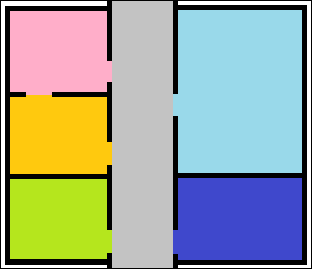
\includegraphics[width=\linewidth]{layout_alg}
\end{minipage}

\section[RFID]{De RFID opstellingen}
\label{ch:rfid}

\subsection{Statisch}

\subsubsection{1 antenne aan deurlijst}
\begin{minipage}{0.65\textwidth}
Deze opstelling is de eenvoudigste en 1 van de opstellingen die momenteel wordt gebruikt door Aucxis, ze is voornamelijk opgenomen in dit onderzoek als referentie. Het concept bij deze opstelling is dat aan elke deurlijst 1 RFID antenne hangt. Als er een tag voorbij de antenne gaat registreert deze dit en weten we dar er een beweging heeft plaatsgevonden. Of deze in of uit de locatie is kan niet uit deze data alleen afgeleid worden, dit kan enkel in combinatie met de informatie wat zijn locatie was voor de verplaatsing. Dit is een nadeel aan deze opstelling.
\end{minipage}
\hfill
\begin{minipage}{0.30\textwidth}
	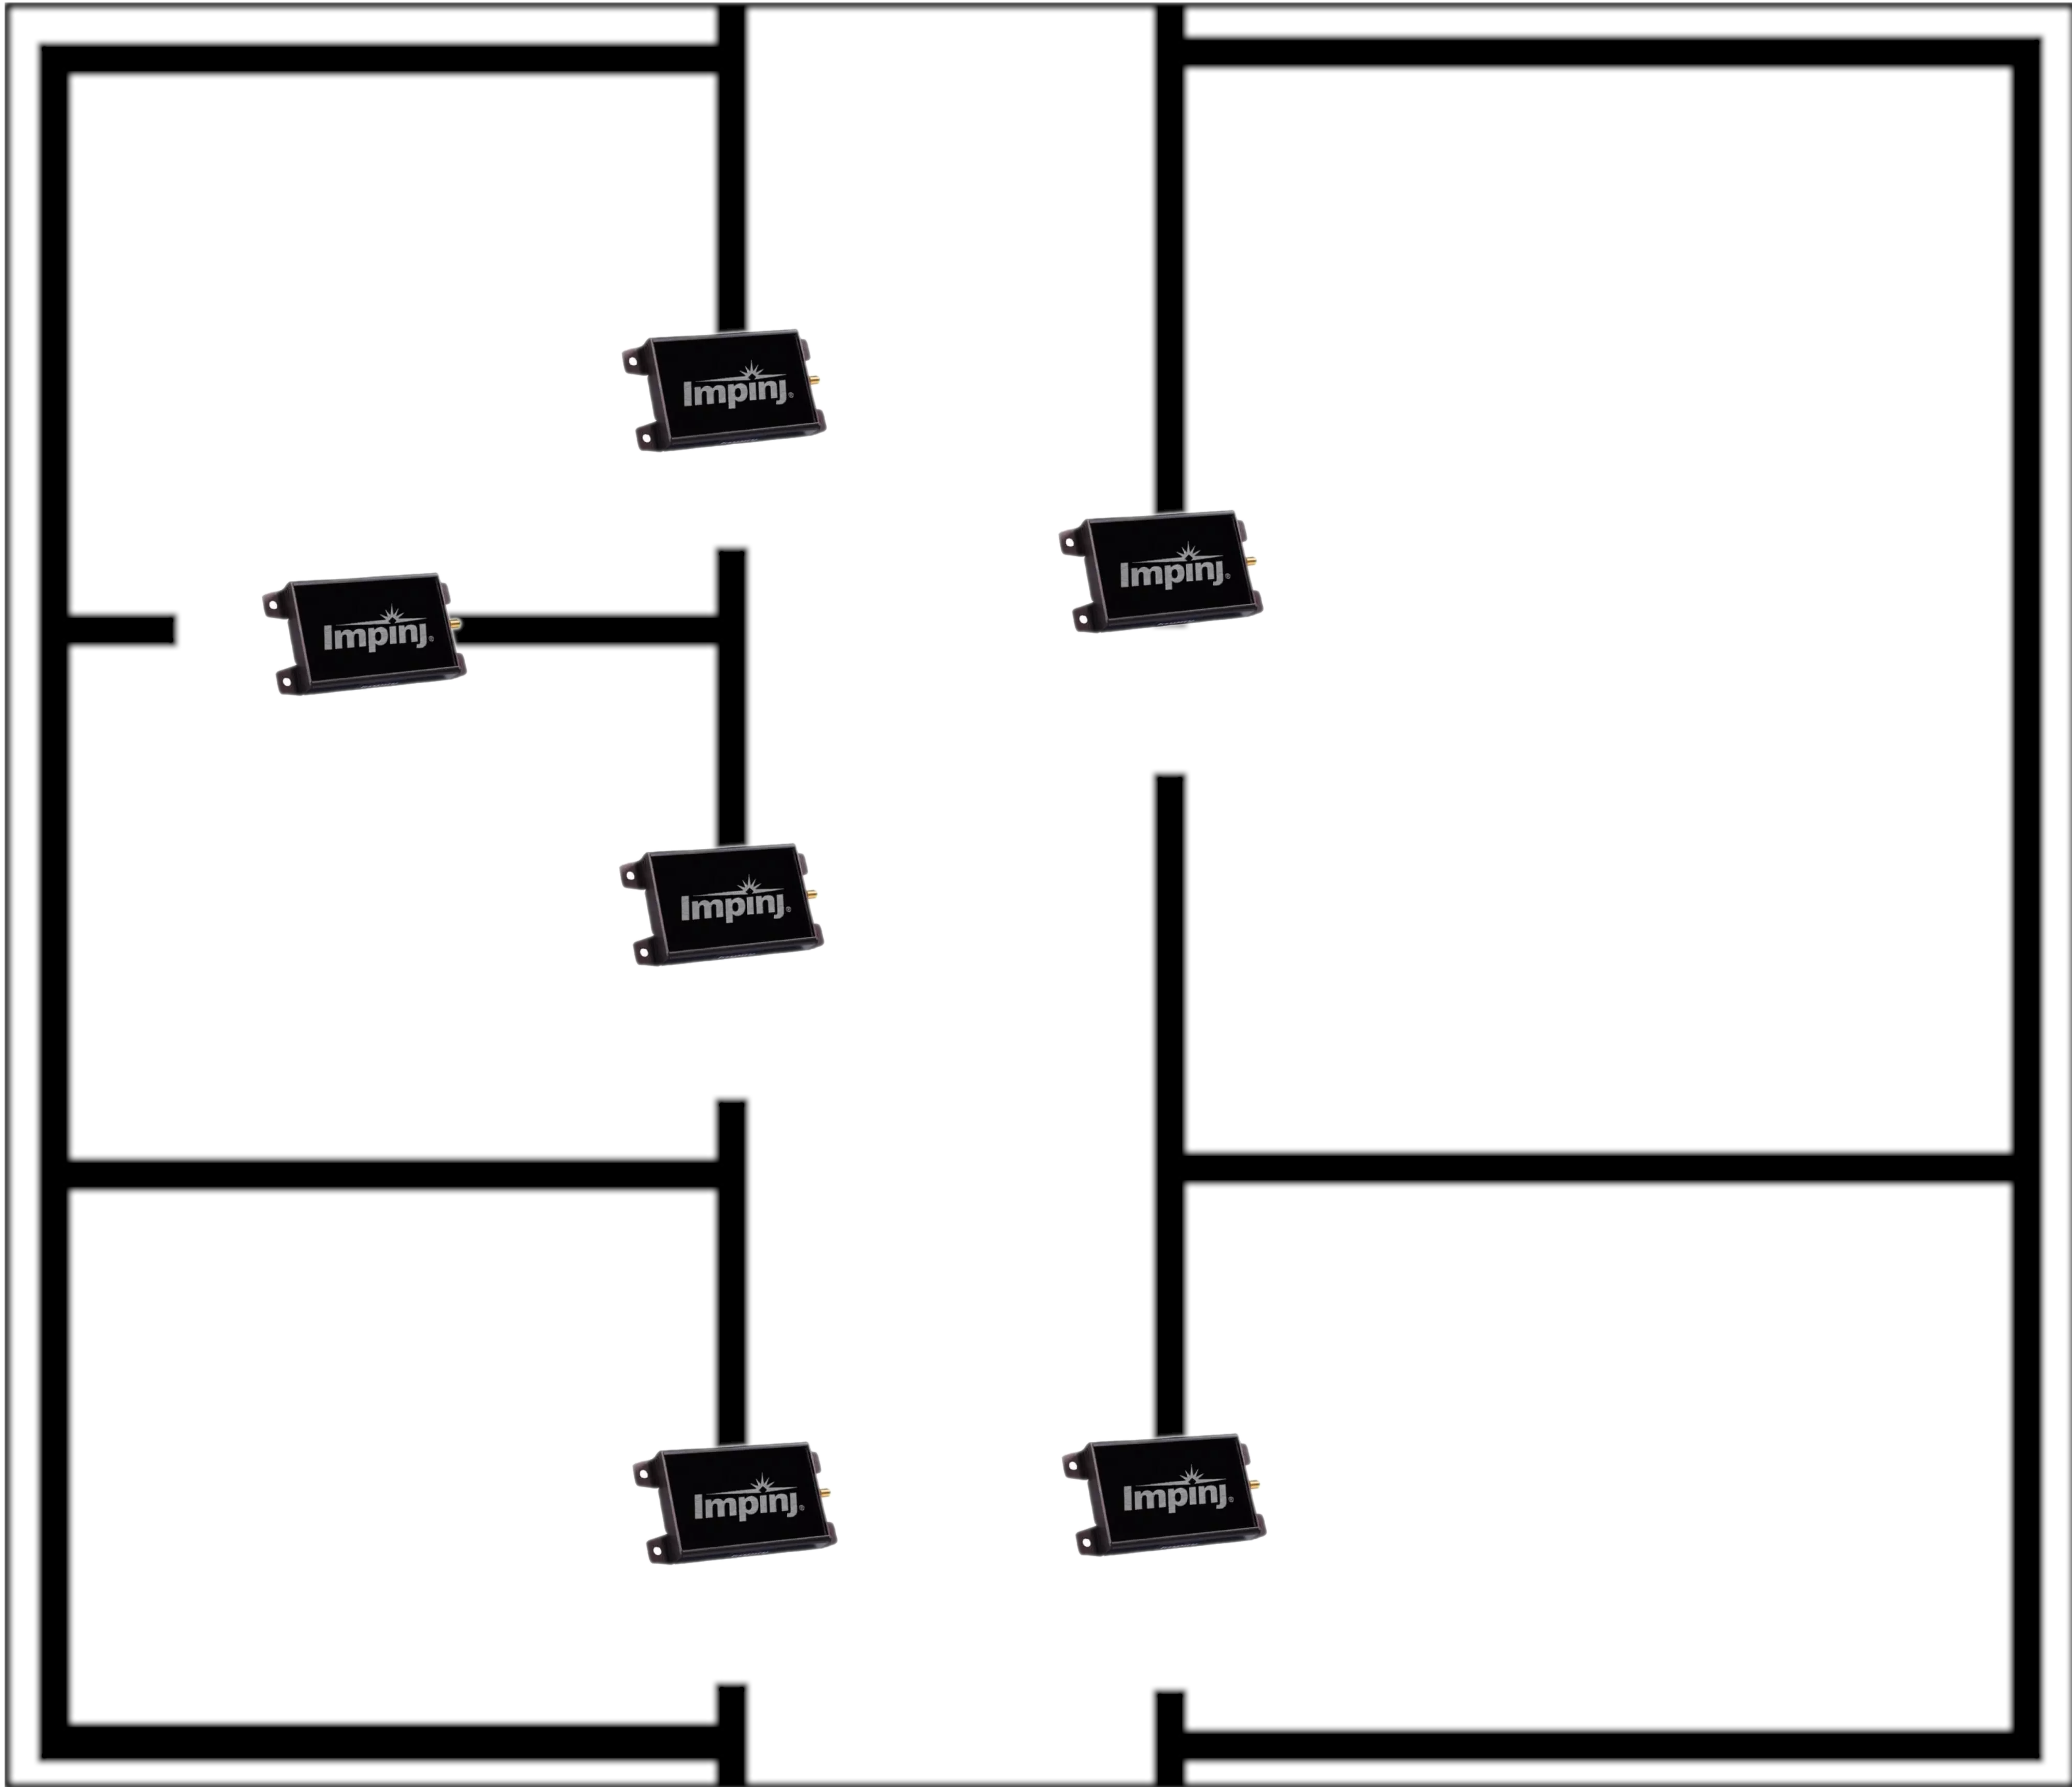
\includegraphics[width=\linewidth]{rfid_static_1}
\end{minipage}

\subsubsection{2 antenne aan deurlijst}
\begin{minipage}{0.65\textwidth}
Dit is ook 1 van de opstellingen die momenteel wordt gebruikt door Aucxis en dus ook voornamelijk een referentiepunt. Het principe is ongeveer hetzelfde als bij de vorige opstelling, echter is hier het voordeel dat de richting van de verplaatsing wel bekend is aan de hand van het tijdsverschil tussen de detecties van de tag. In dit opzicht is het dus beter dan de vorige opstelling, maar is uiteraard duurder door de hogere aantallen benodigde antennes. 
\end{minipage}
\hfill
\begin{minipage}{0.30\textwidth}
	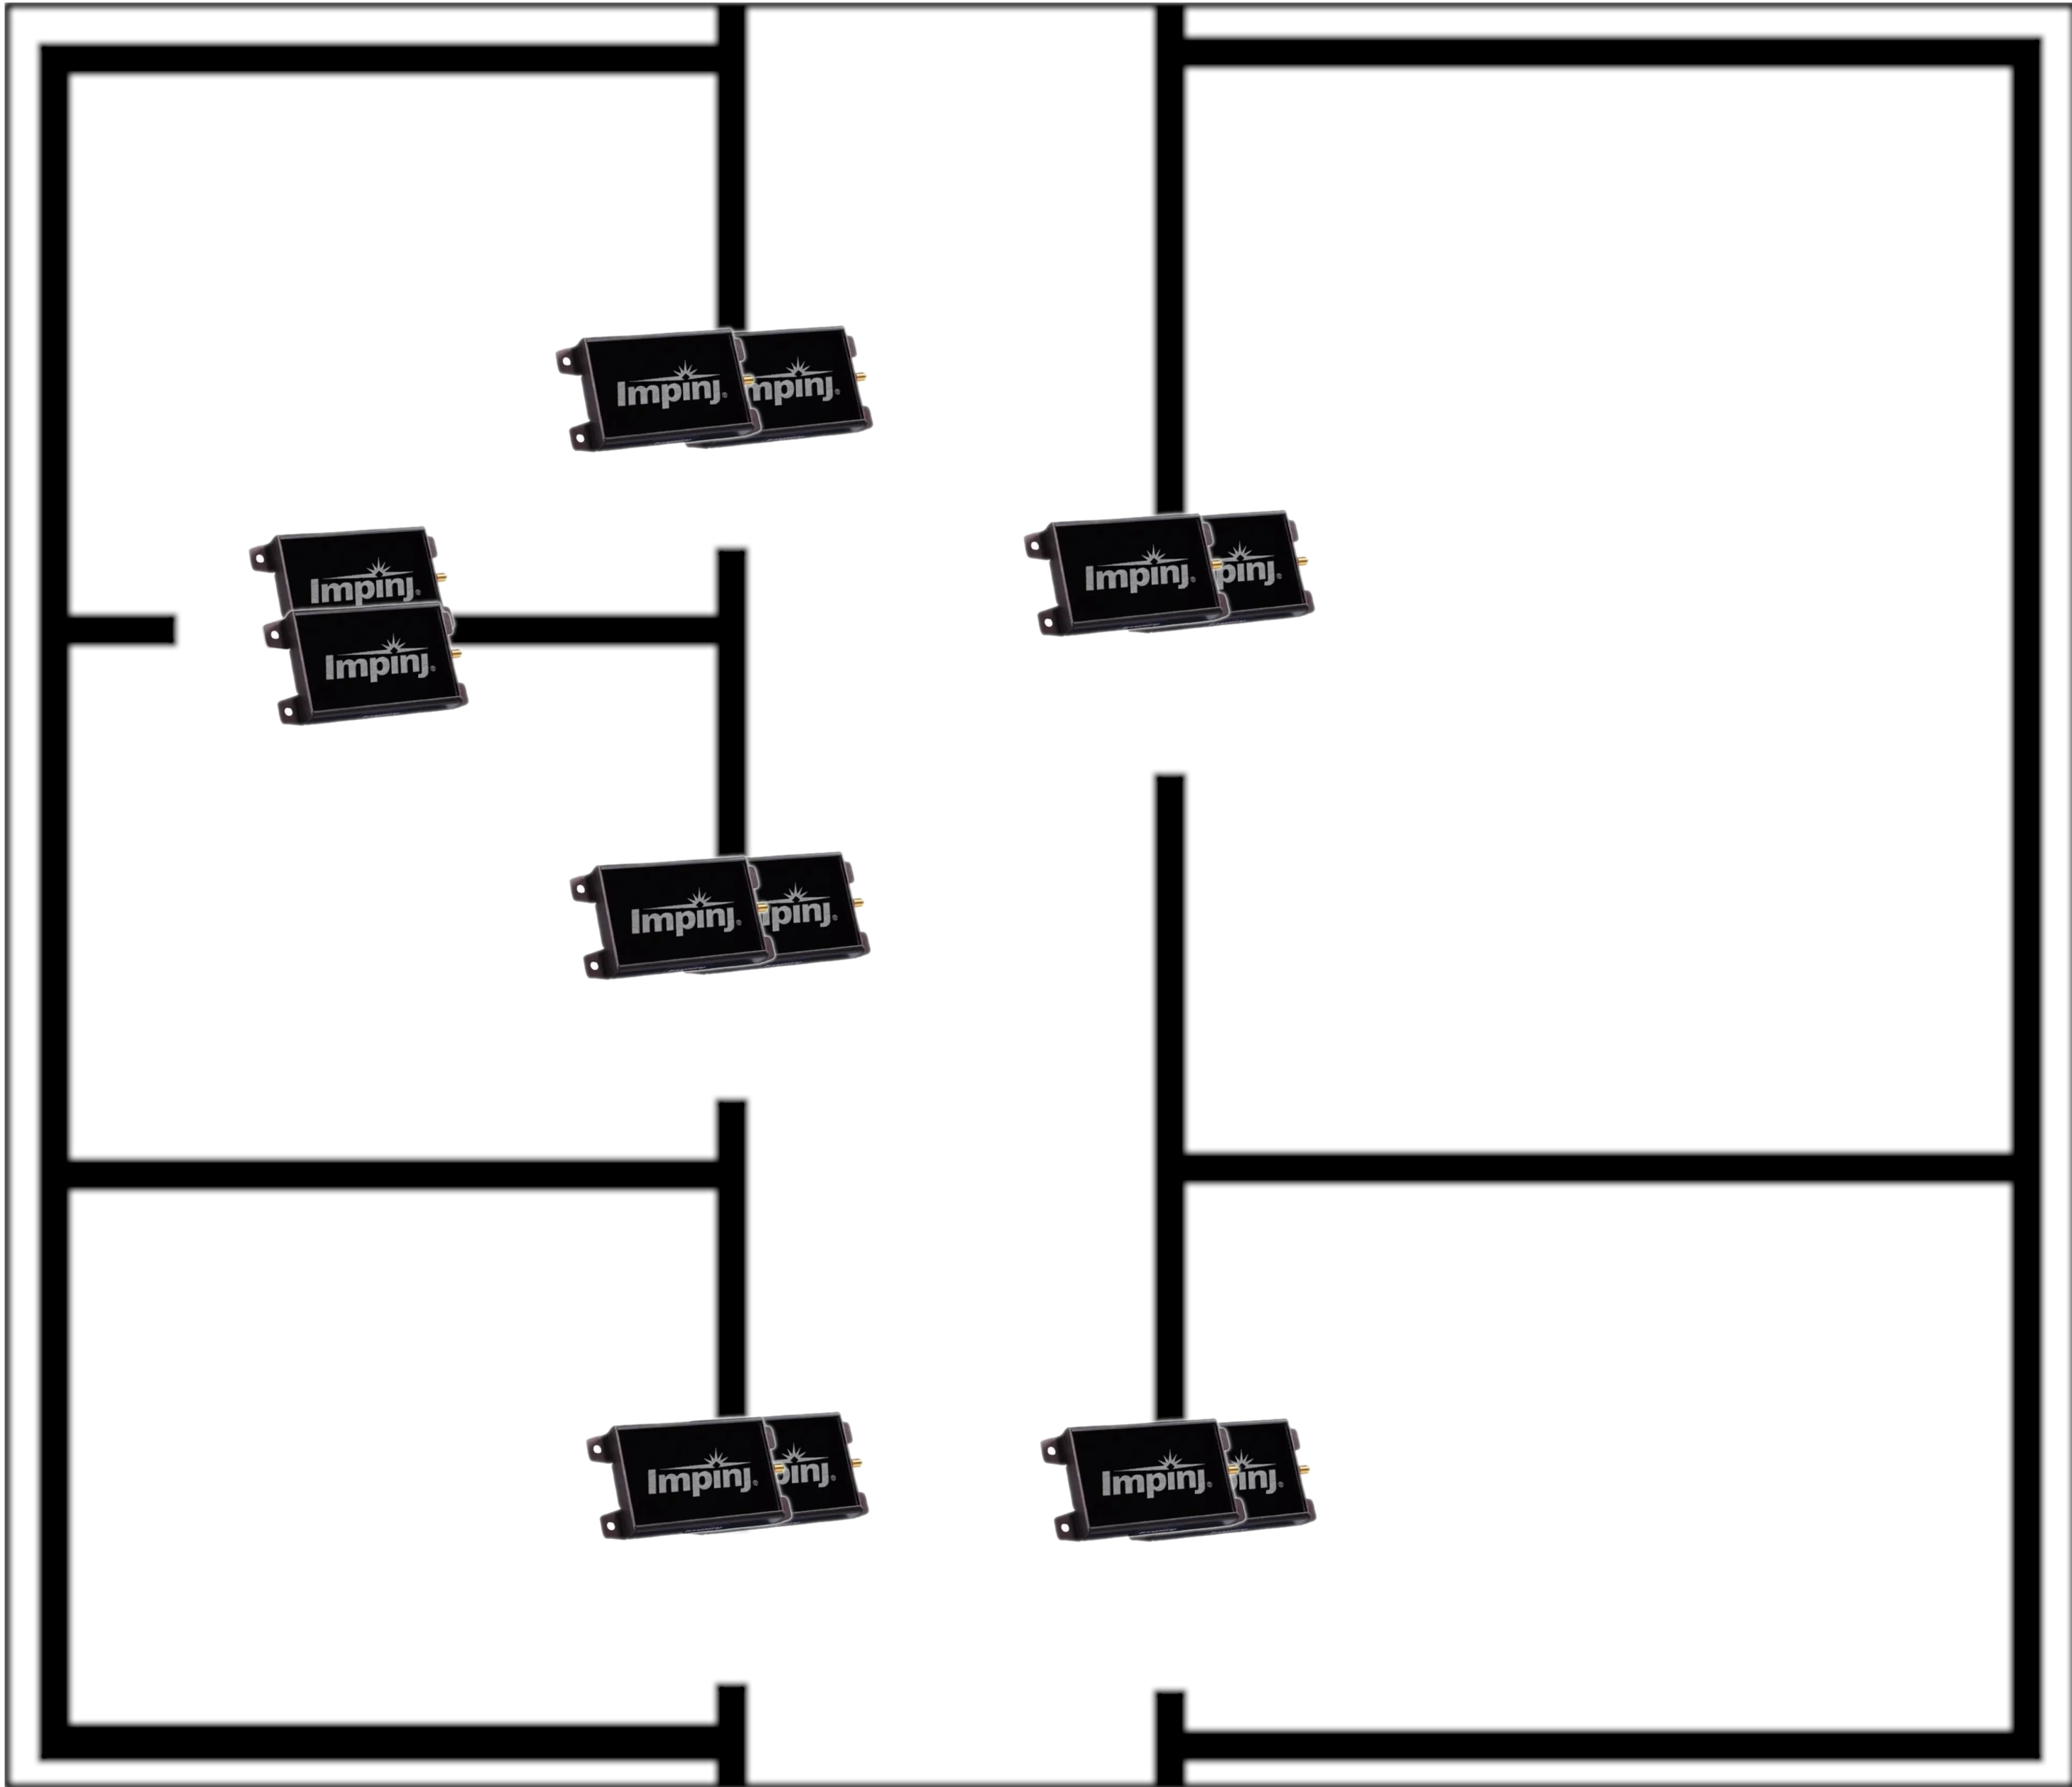
\includegraphics[width=\linewidth]{rfid_static_2}
\end{minipage}

\subsubsection{1 antenne tegenover deur}
\begin{minipage}{0.65\textwidth}
Bij deze opstelling wordt een RFID antenne tegenover de deur geplaatst, het idee hierachter is het feit dat, aangezien de RSSI afhankelijk is van de afstand tussen de antenne en de tag, het in theorie zichtbaar is aan de verandering in RSSI in welke richting de tag gaat. Ook geeft de antenne een doppler waarde mee, welke in theorie ook veranderd naargelang de richting. Als dit in praktijk blijkt te werken wilt dit zeggen dat er richtingsdetectie mogelijk is met 1 antenne, waardoor het sowieso al beter is dan de vorige 2 opstellingen. Nadeel is wel dat de kamer niet te breed mag zijn zodat de antenne ook tegenover de deur kan worden gemonteerd.
\end{minipage}
\hfill
\begin{minipage}{0.30\textwidth}
	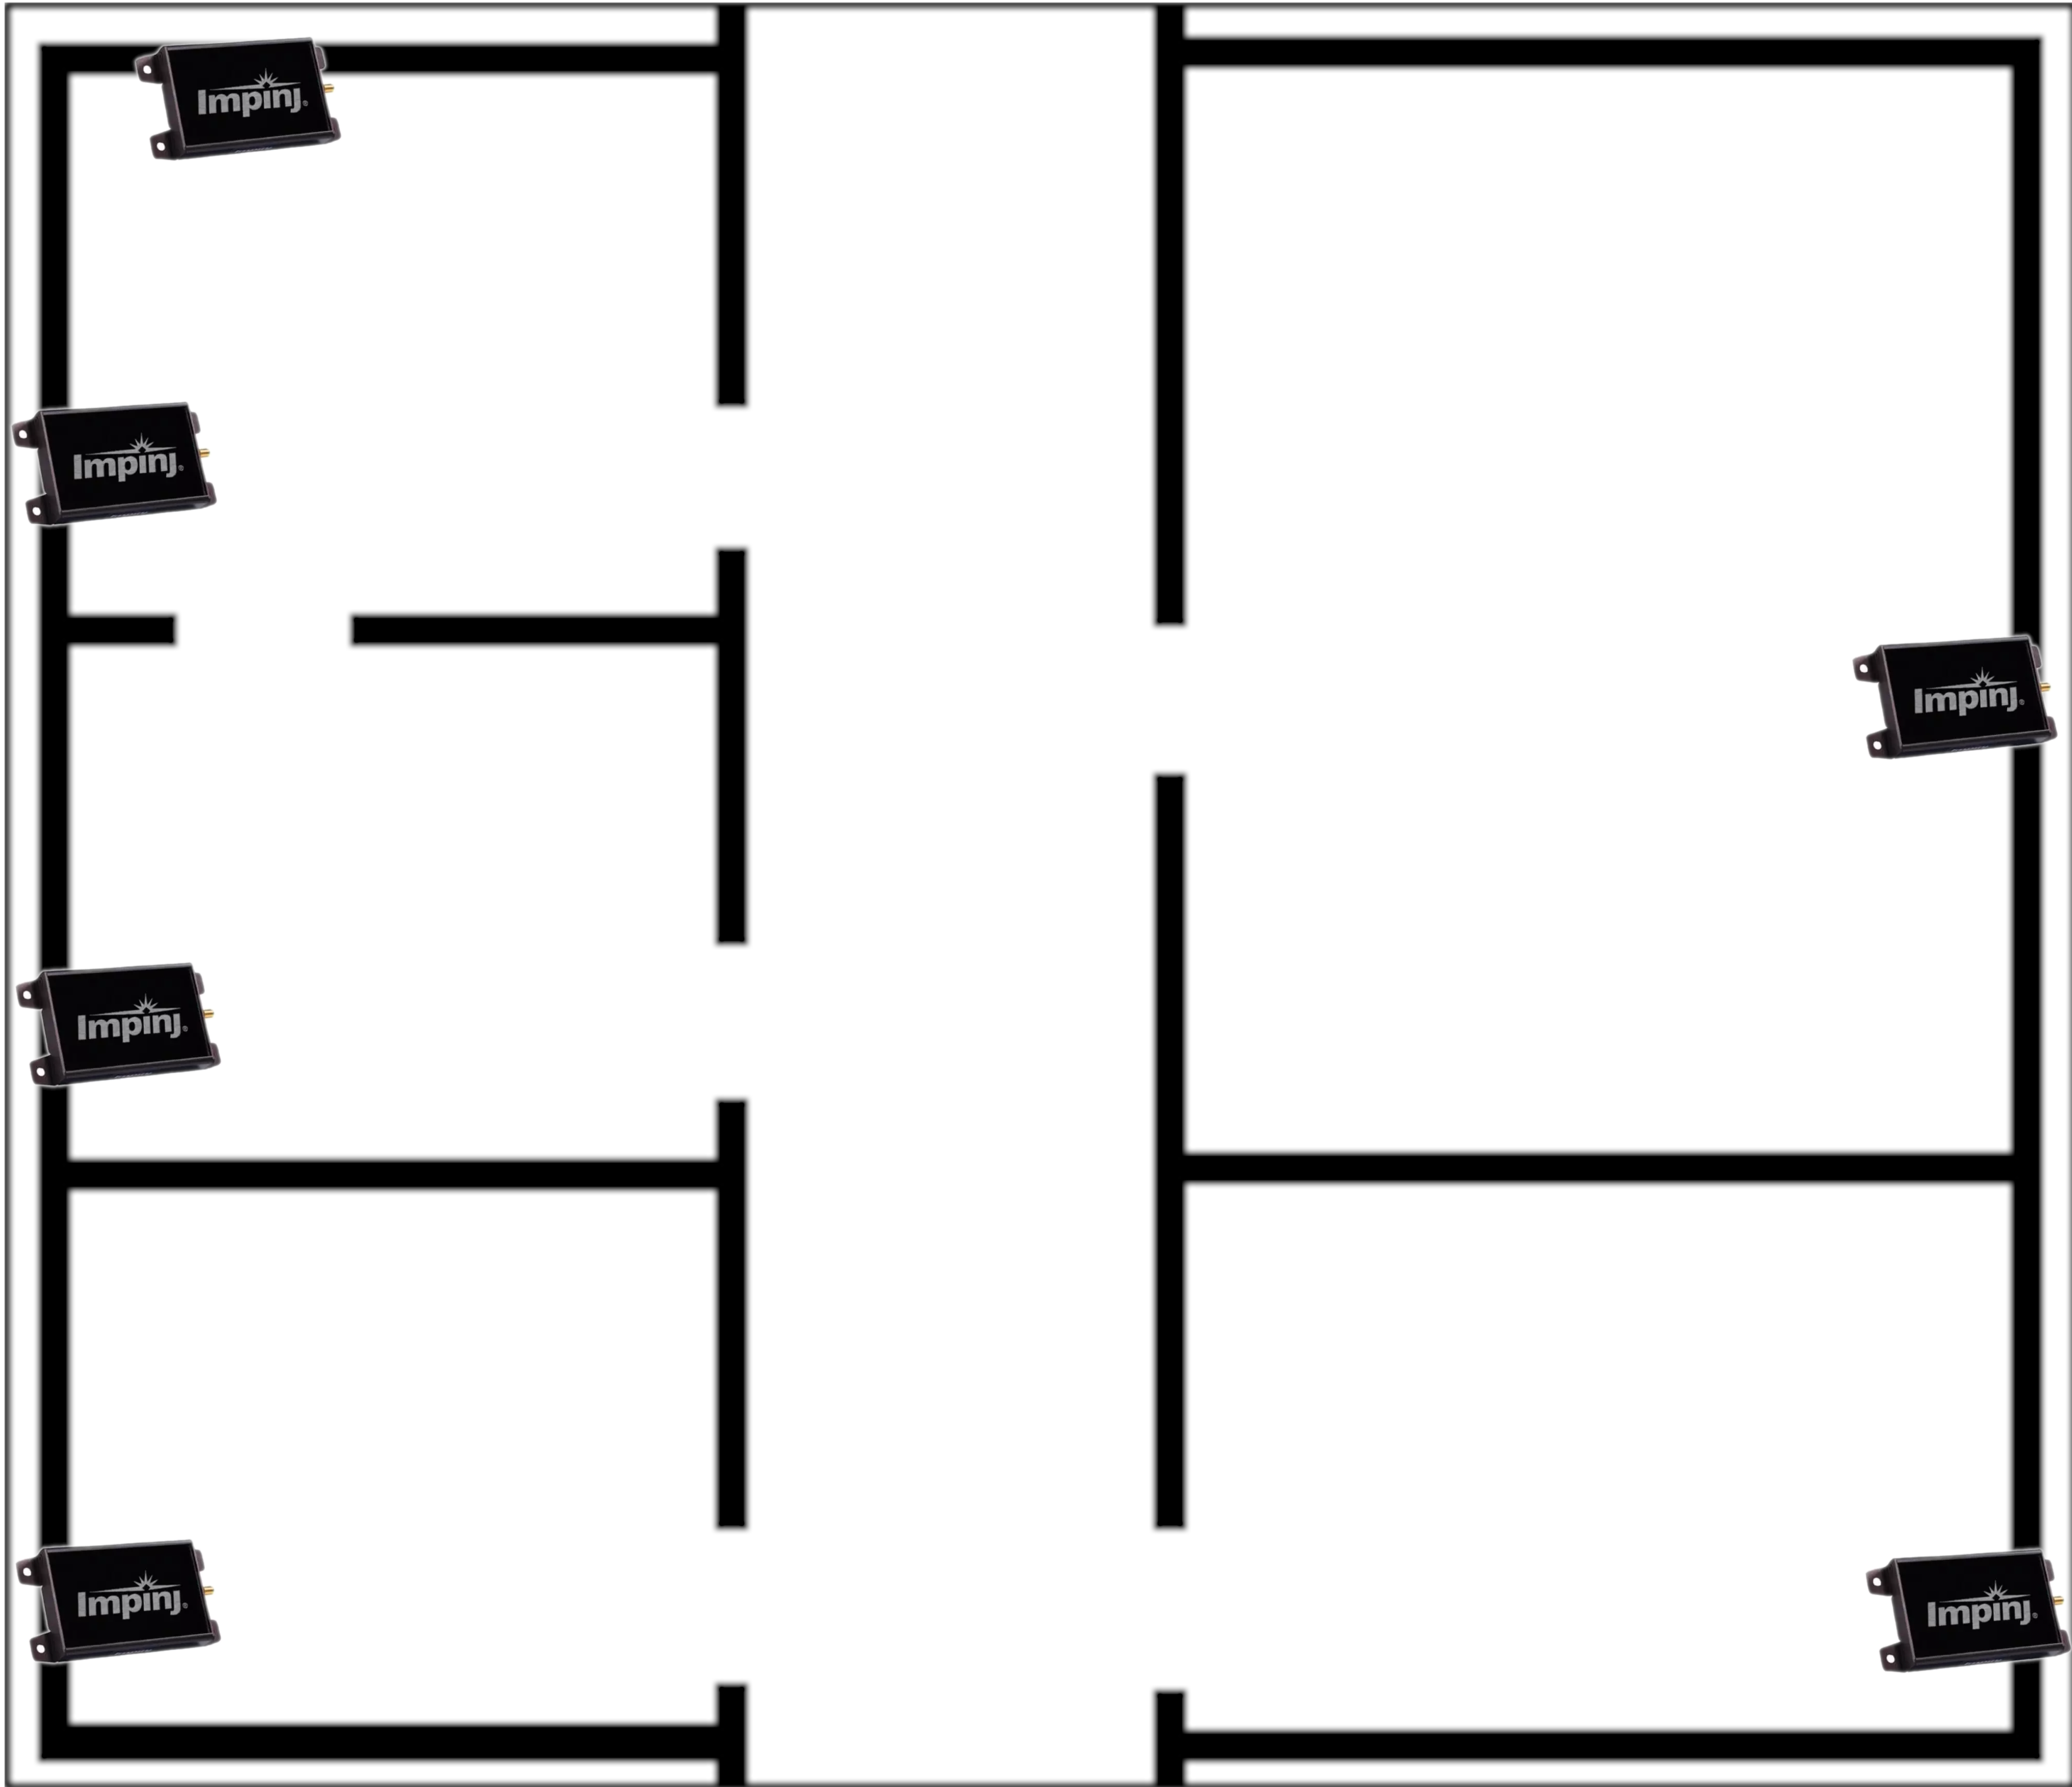
\includegraphics[width=\linewidth]{rfid_static_3}
\end{minipage}
\subsection{Dynamisch}

\subsubsection{1 tag aan deurlijst}
\begin{minipage}{0.65\textwidth}
Hier hangt er een RFID-tag aan de deurlijst (analoog aan de antenne bij de eerste statische opstelling). Als de antenne passeert aan de deur weet het aggregatieprogramma in theorie dat alle tags tussen nu en het passeren van deze of een andere locatie RFID-tag tot deze locatie behoren.
\end{minipage}
\hfill
\begin{minipage}{0.30\textwidth}
	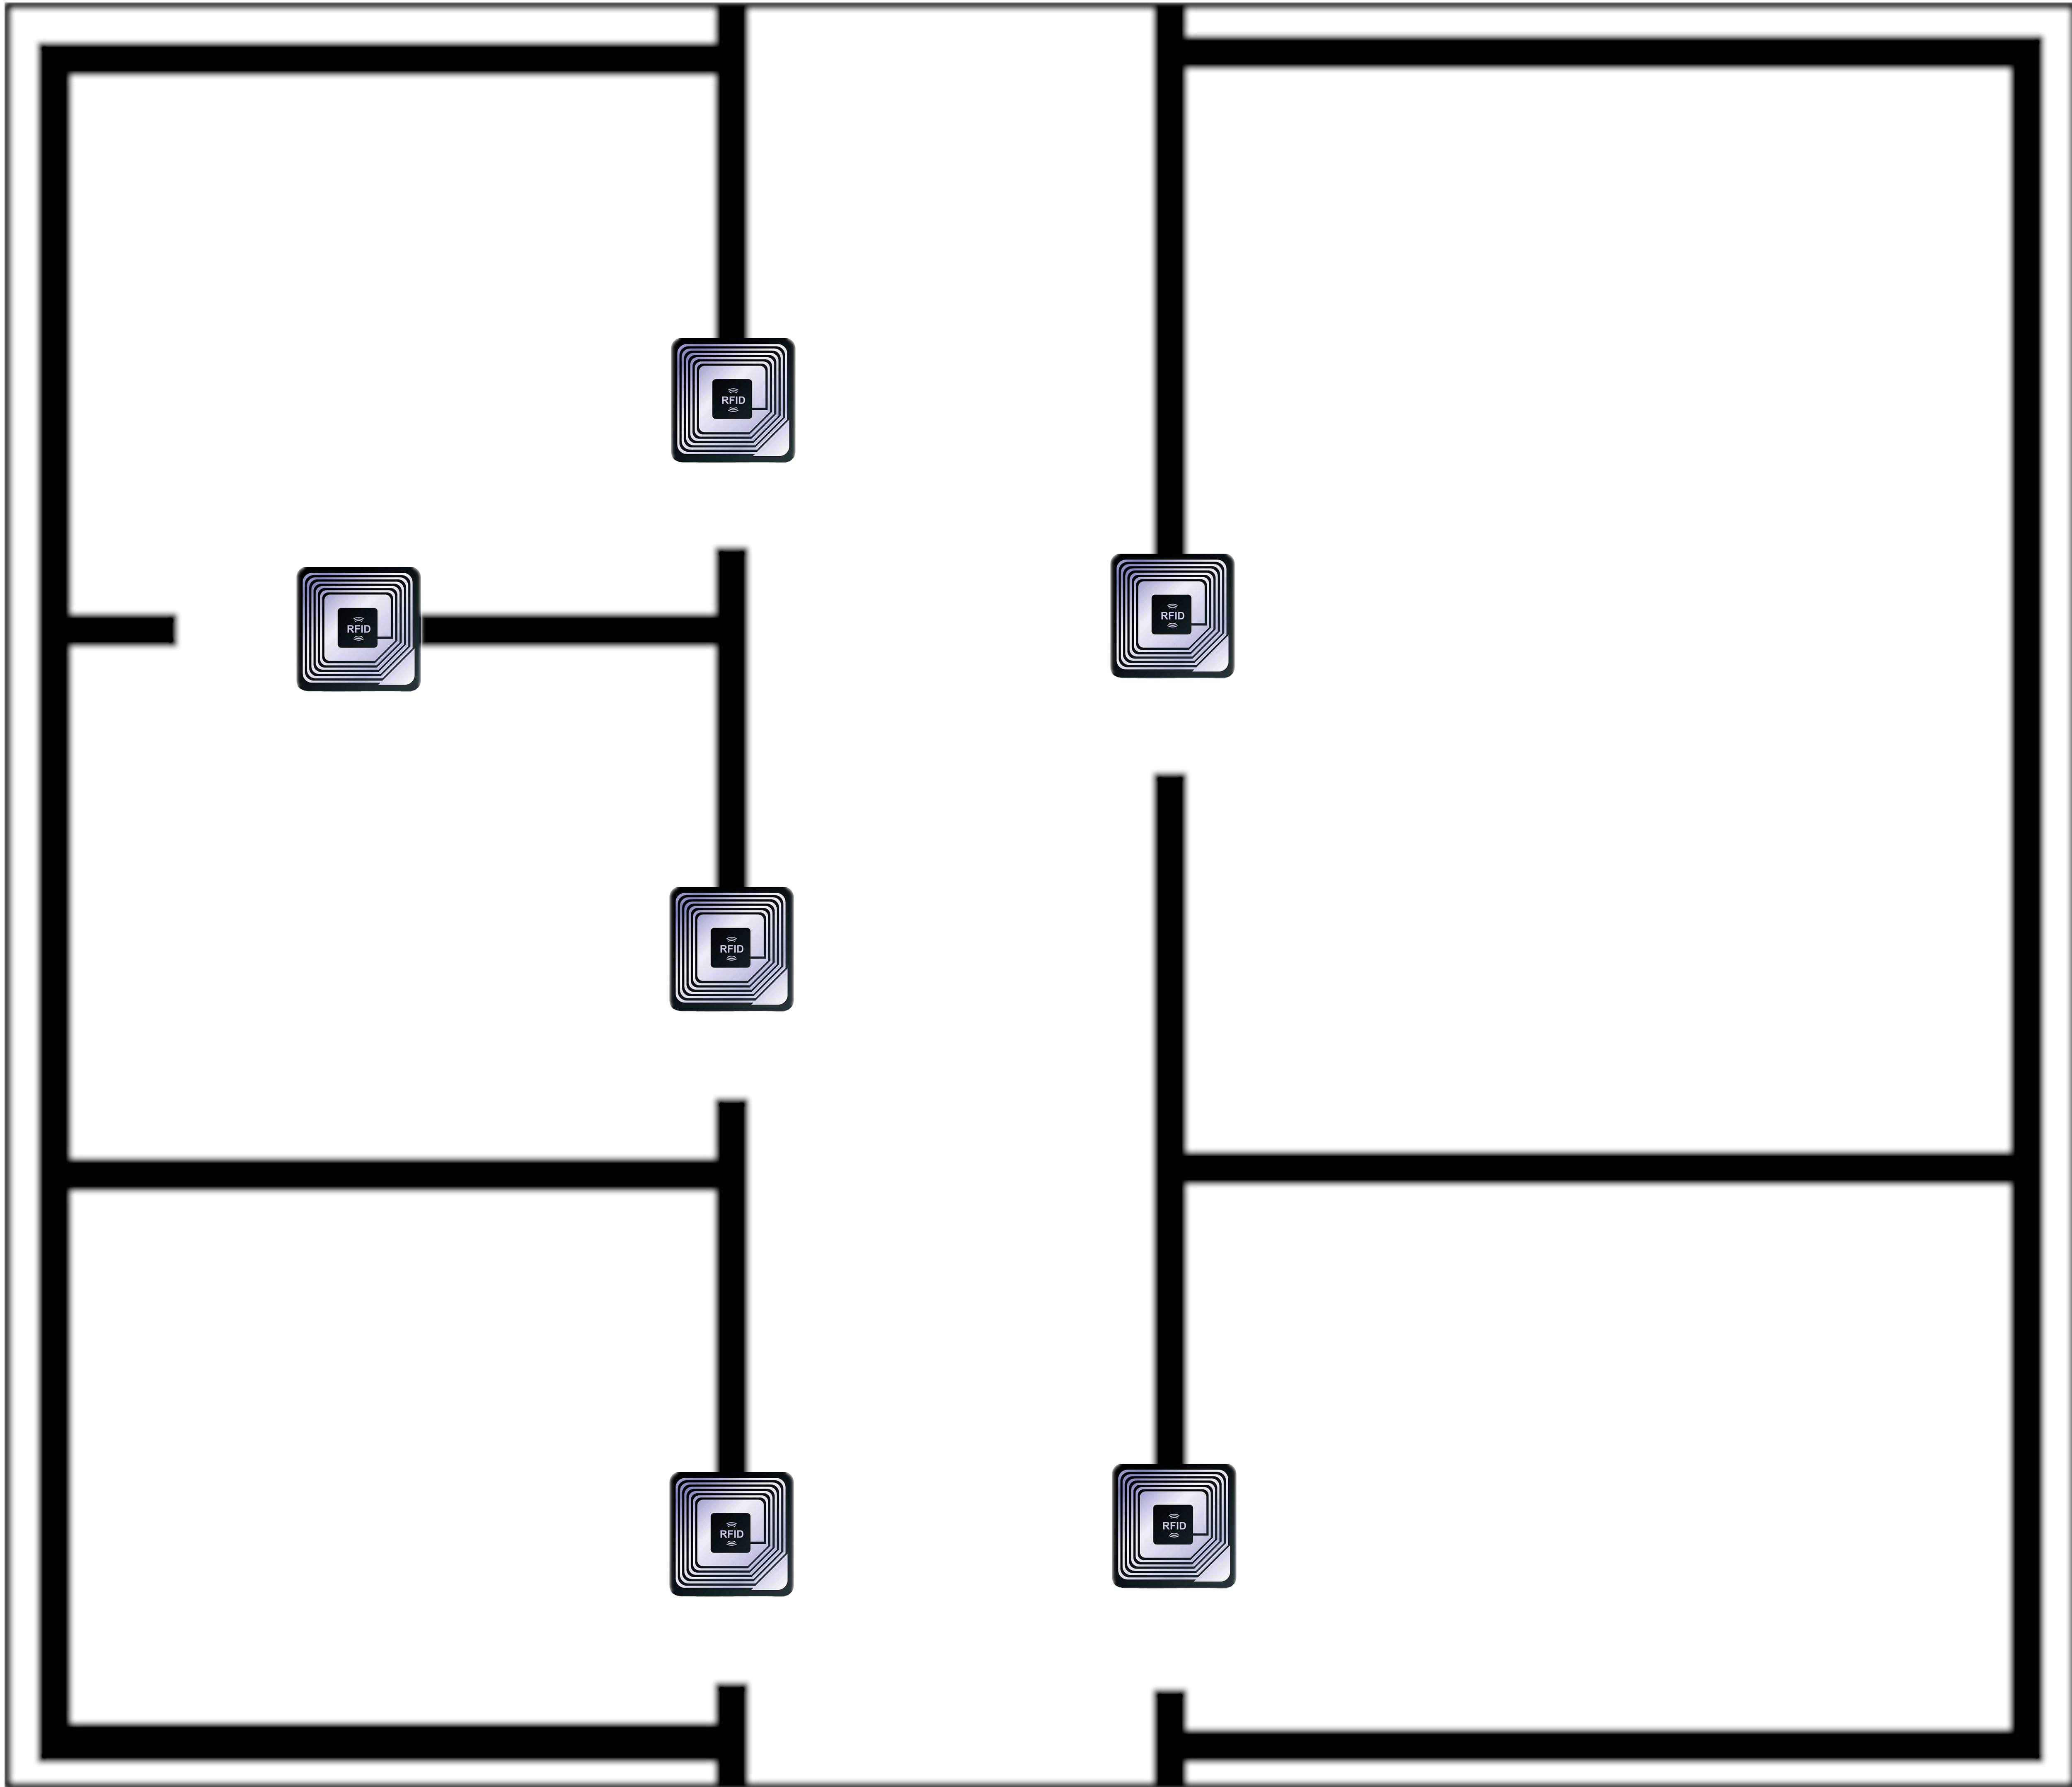
\includegraphics[width=\linewidth]{rfid_dynamic_1}
\end{minipage}

In theorie is het ook mogelijk de 2 andere statische scenario's een dynamische variant te geven, echter valt hun voordeel van richtingbepalend zijn weg hierbij aangezien de richting niet meer relevant is bij dynamisch. Deze worden dus buiten beschouwing gelaten.

\section[BLE]{De BLE opstellingen}
\label{ch:ble}

\subsection{Statisch}

\subsubsection{1 gateway per locatie}
\begin{minipage}{0.65\textwidth}
Deze opstelling is de eenvoudigste en meest intuïtieve van de BLE opstellingen. Elke locatie komt overeen met 1 IoT Gateway, die gepositioneerd wordt ongeveer in het middelpunt van de locatie. Het idee hierachter is dat de Gateway waar de beacon het dichtste bij is (de beste RSSI heeft), hoogstwaarschijnlijk de locatie is waar het voorwerp zich bevind. Dit is echter niet 100\% correct, en deze onnauwkeurigheid zal enkel maar groeien als de gateways/locaties onevenredig verdeeld zijn over de oppervlakte van het gebouw. 
\end{minipage}
\hfill
\begin{minipage}{0.30\textwidth}
	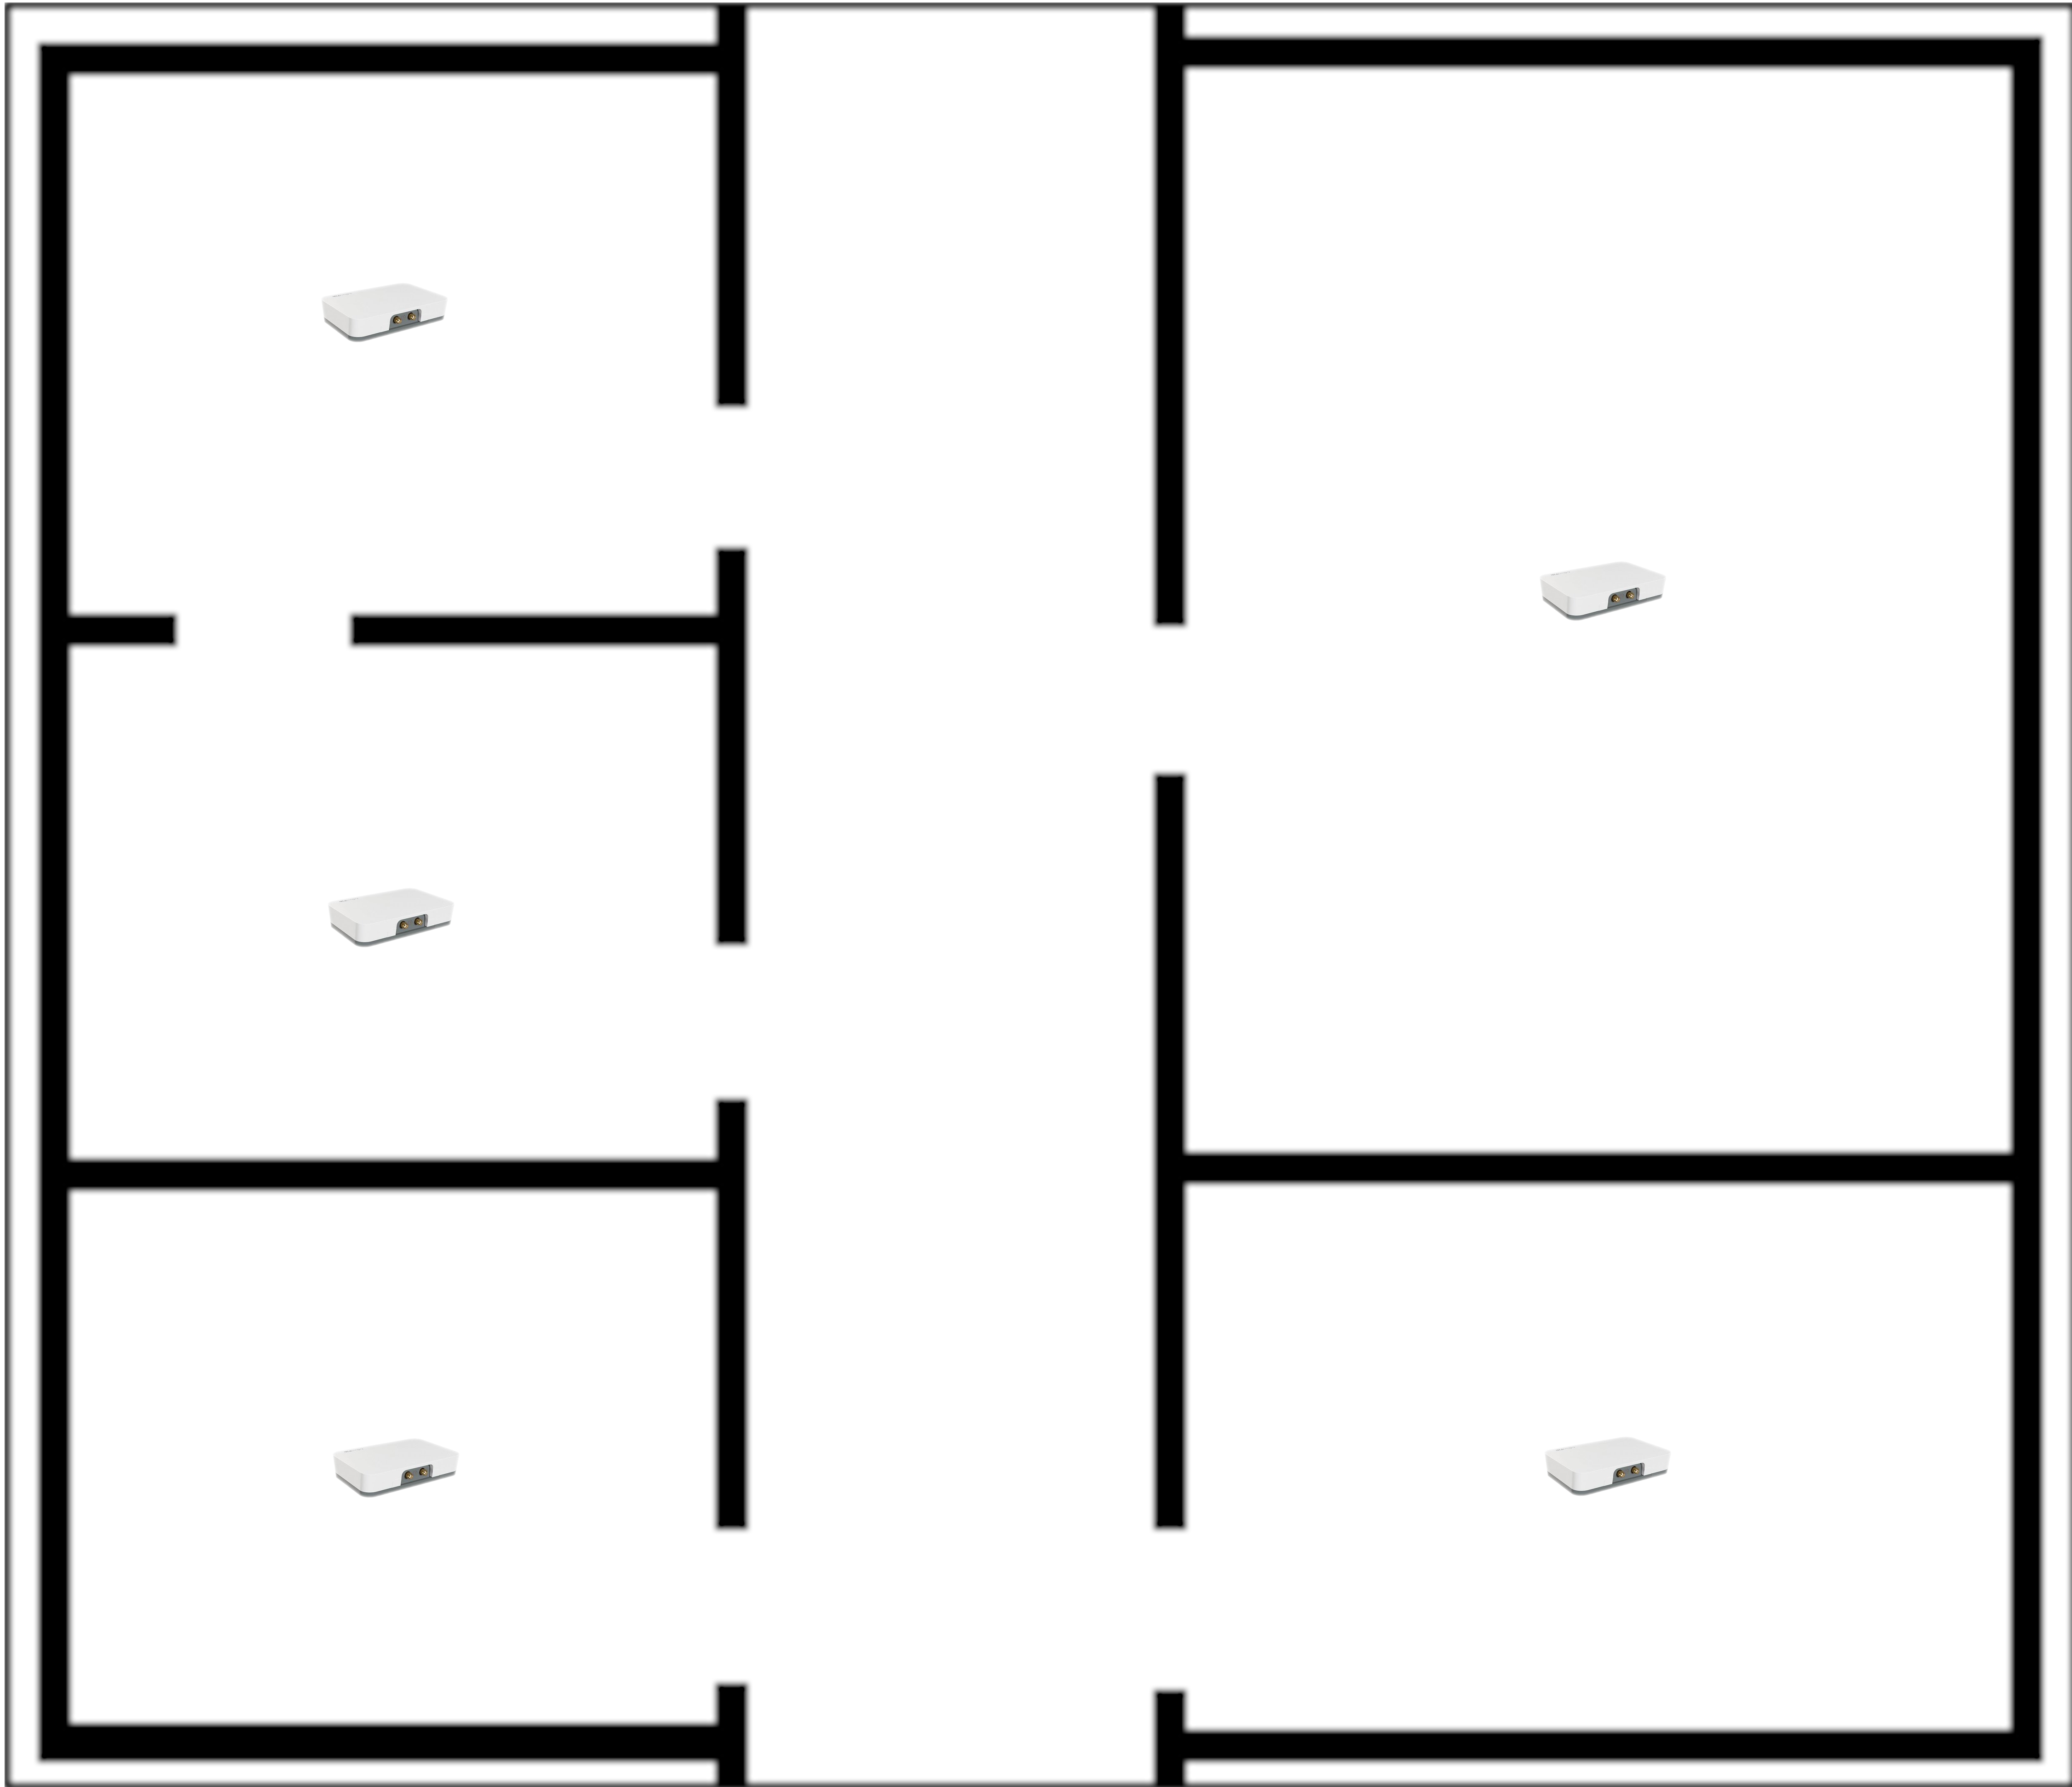
\includegraphics[width=\linewidth]{ble_statisch_1}
\end{minipage}

\subsubsection{Meerdere gateways per locatie}
\begin{minipage}{0.65\textwidth}
In deze opstelling wordt een locatie gedefinieerd door meer dan 1 gateway, nl. een gateway per hoek van de locatie, zodat de locatie wordt omringd door een kader van gateways. Hiermee kan in theorie zeer gedetailleerd worden afgeleid waar de beacon zich bevind, maar de kost voor de opstelling vliegt vrij snel de hoogte in als er veel locaties zijn. Wel kunnen gedeelde hoeken van locaties door een gedeelde beacon worden bezet.
\end{minipage}
\hfill
\begin{minipage}{0.30\textwidth}
	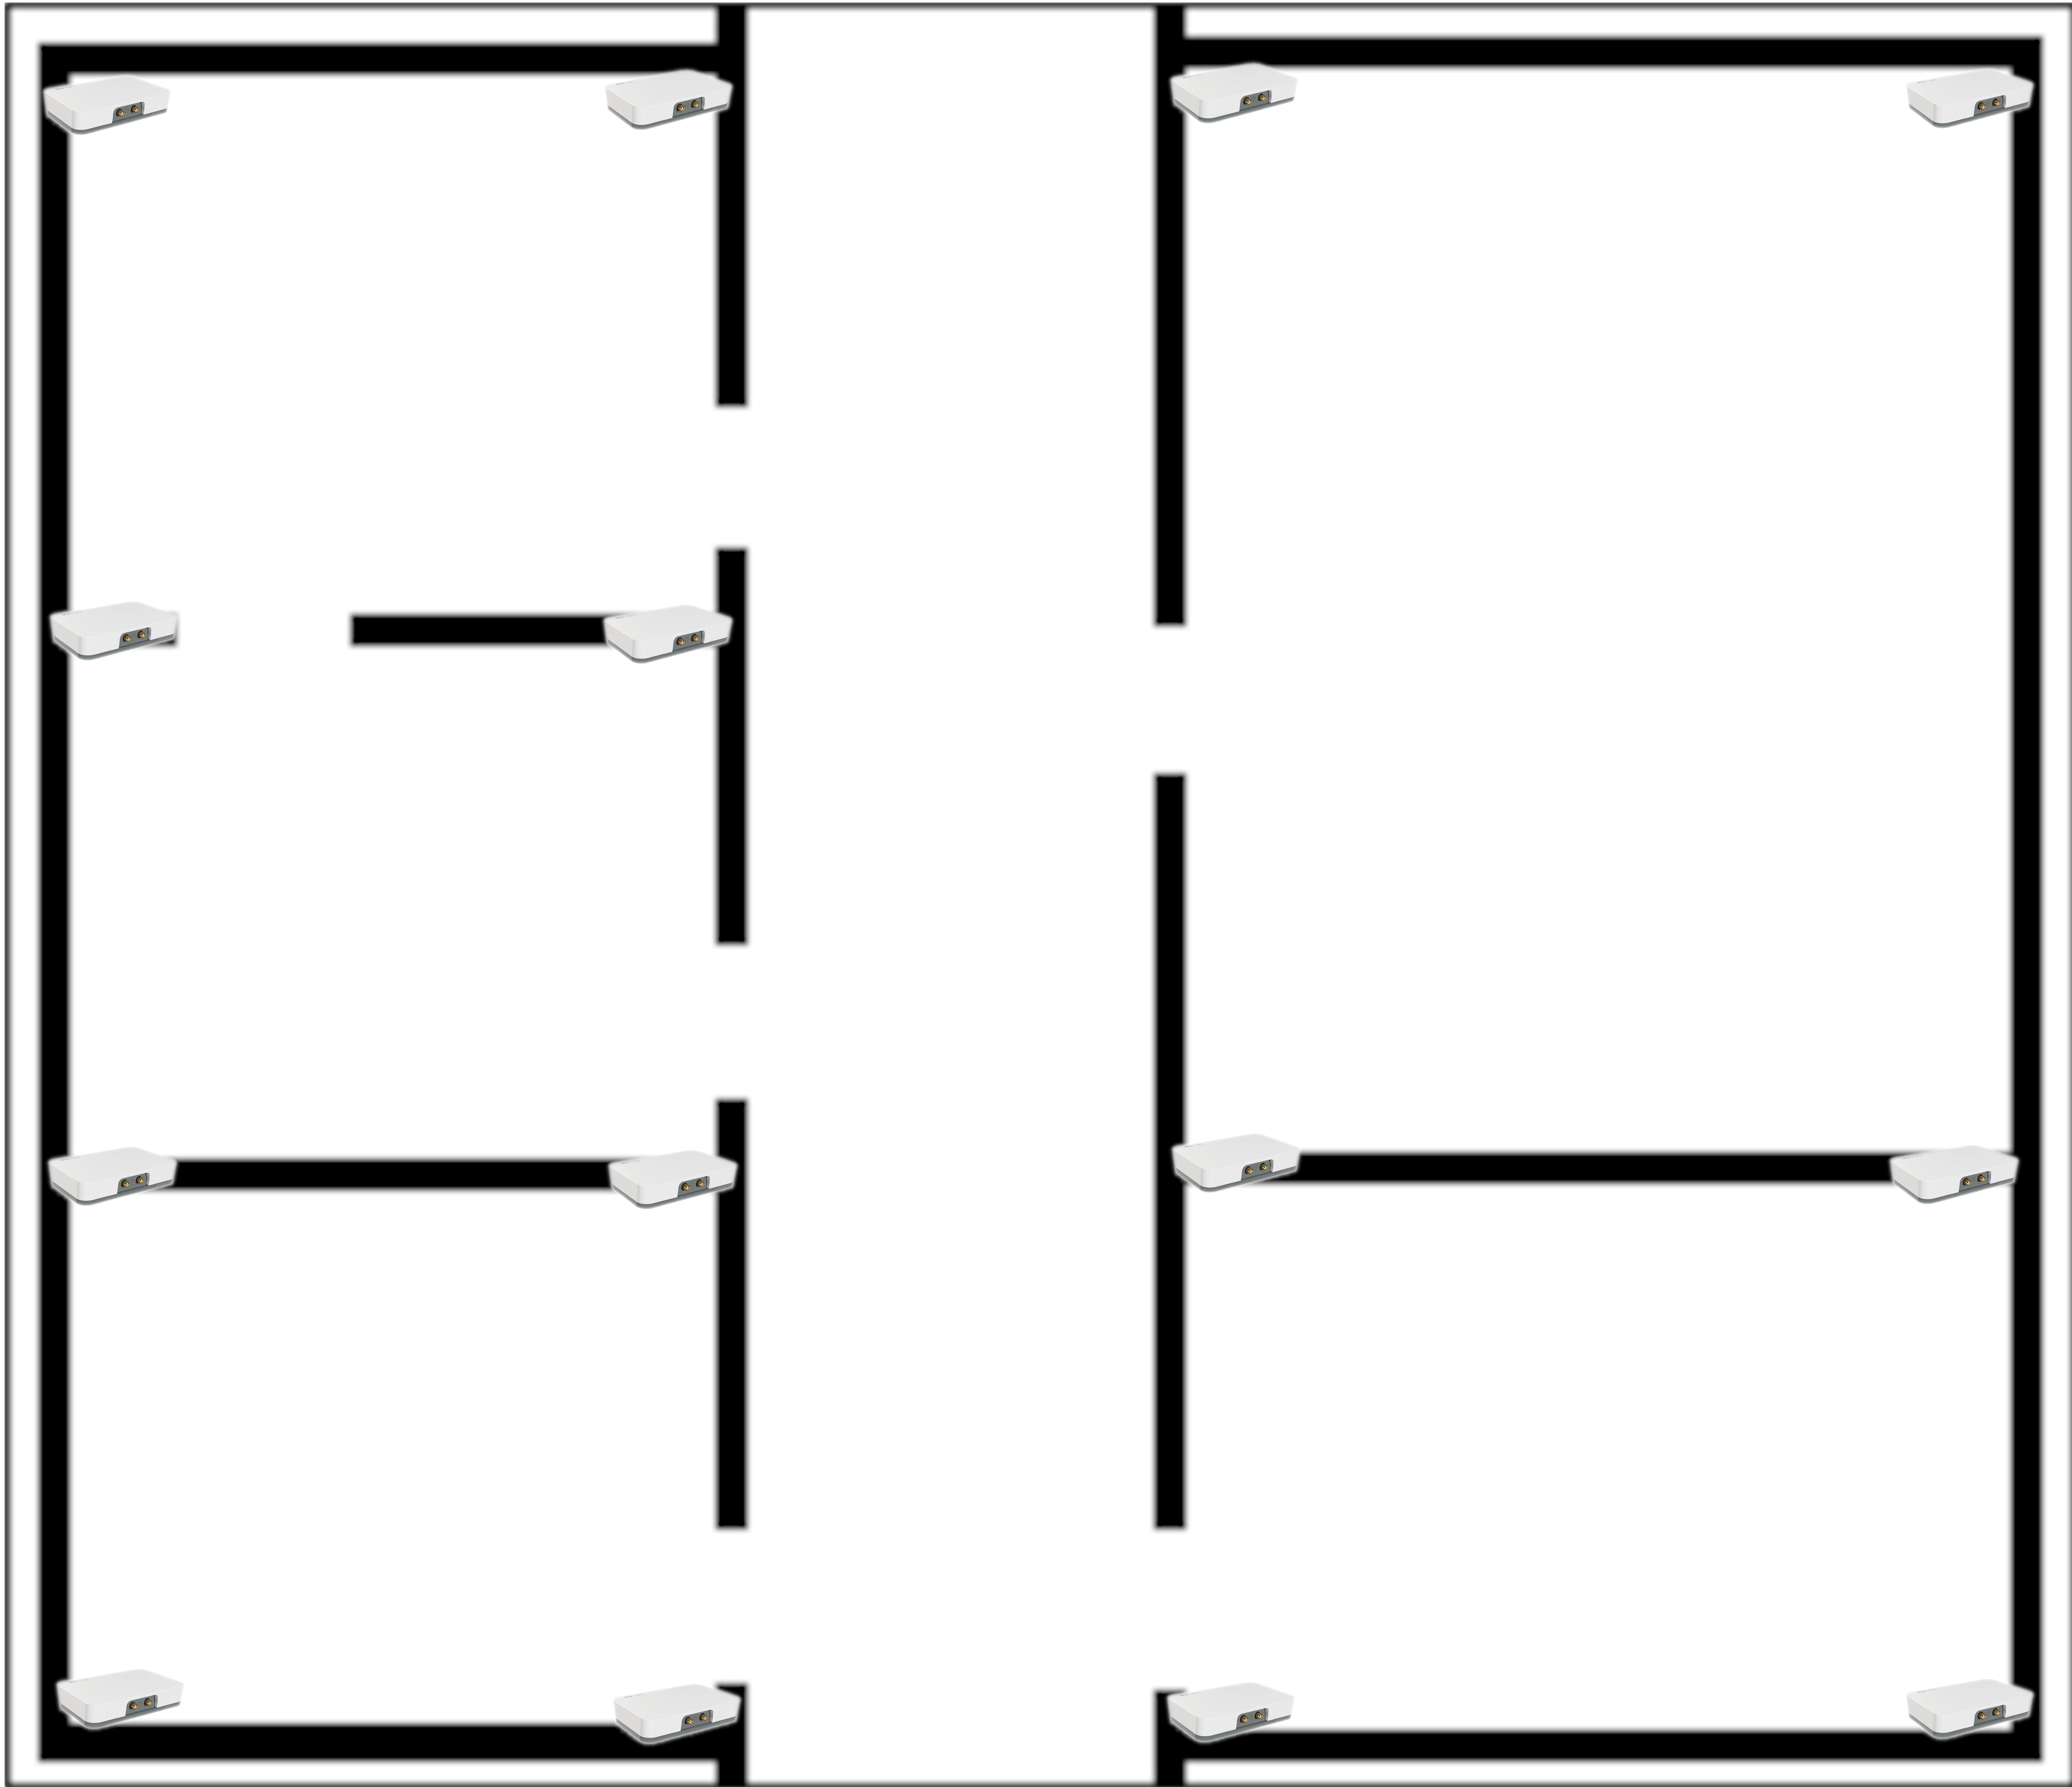
\includegraphics[width=\linewidth]{ble_statisch_2}
\end{minipage}

\subsubsection{Rasteropstelling}
\begin{minipage}{0.65\textwidth}
Deze opstelling bestaat uit een raster welke volledig het gebouw omvat. Als de locaties van deze gateways bekend zijn kan via trigonometrie en de gemeten RSSI waardes berekend worden waar de voorwerpen zich bevinden, wat dan gelinkt kan worden aan een locatie. Dit is vrij precies en schaalt goed, maar nadelig is wel dat de locaties volledig gespecificeerd en bijgehouden moeten worden want er kan niet enkel op data van de gateways worden afgegaan om de locatie te bepalen aangezien de gateways en de locaties niks meer met elkaar te maken hebben.
\end{minipage}
\hfill
\begin{minipage}{0.30\textwidth}
	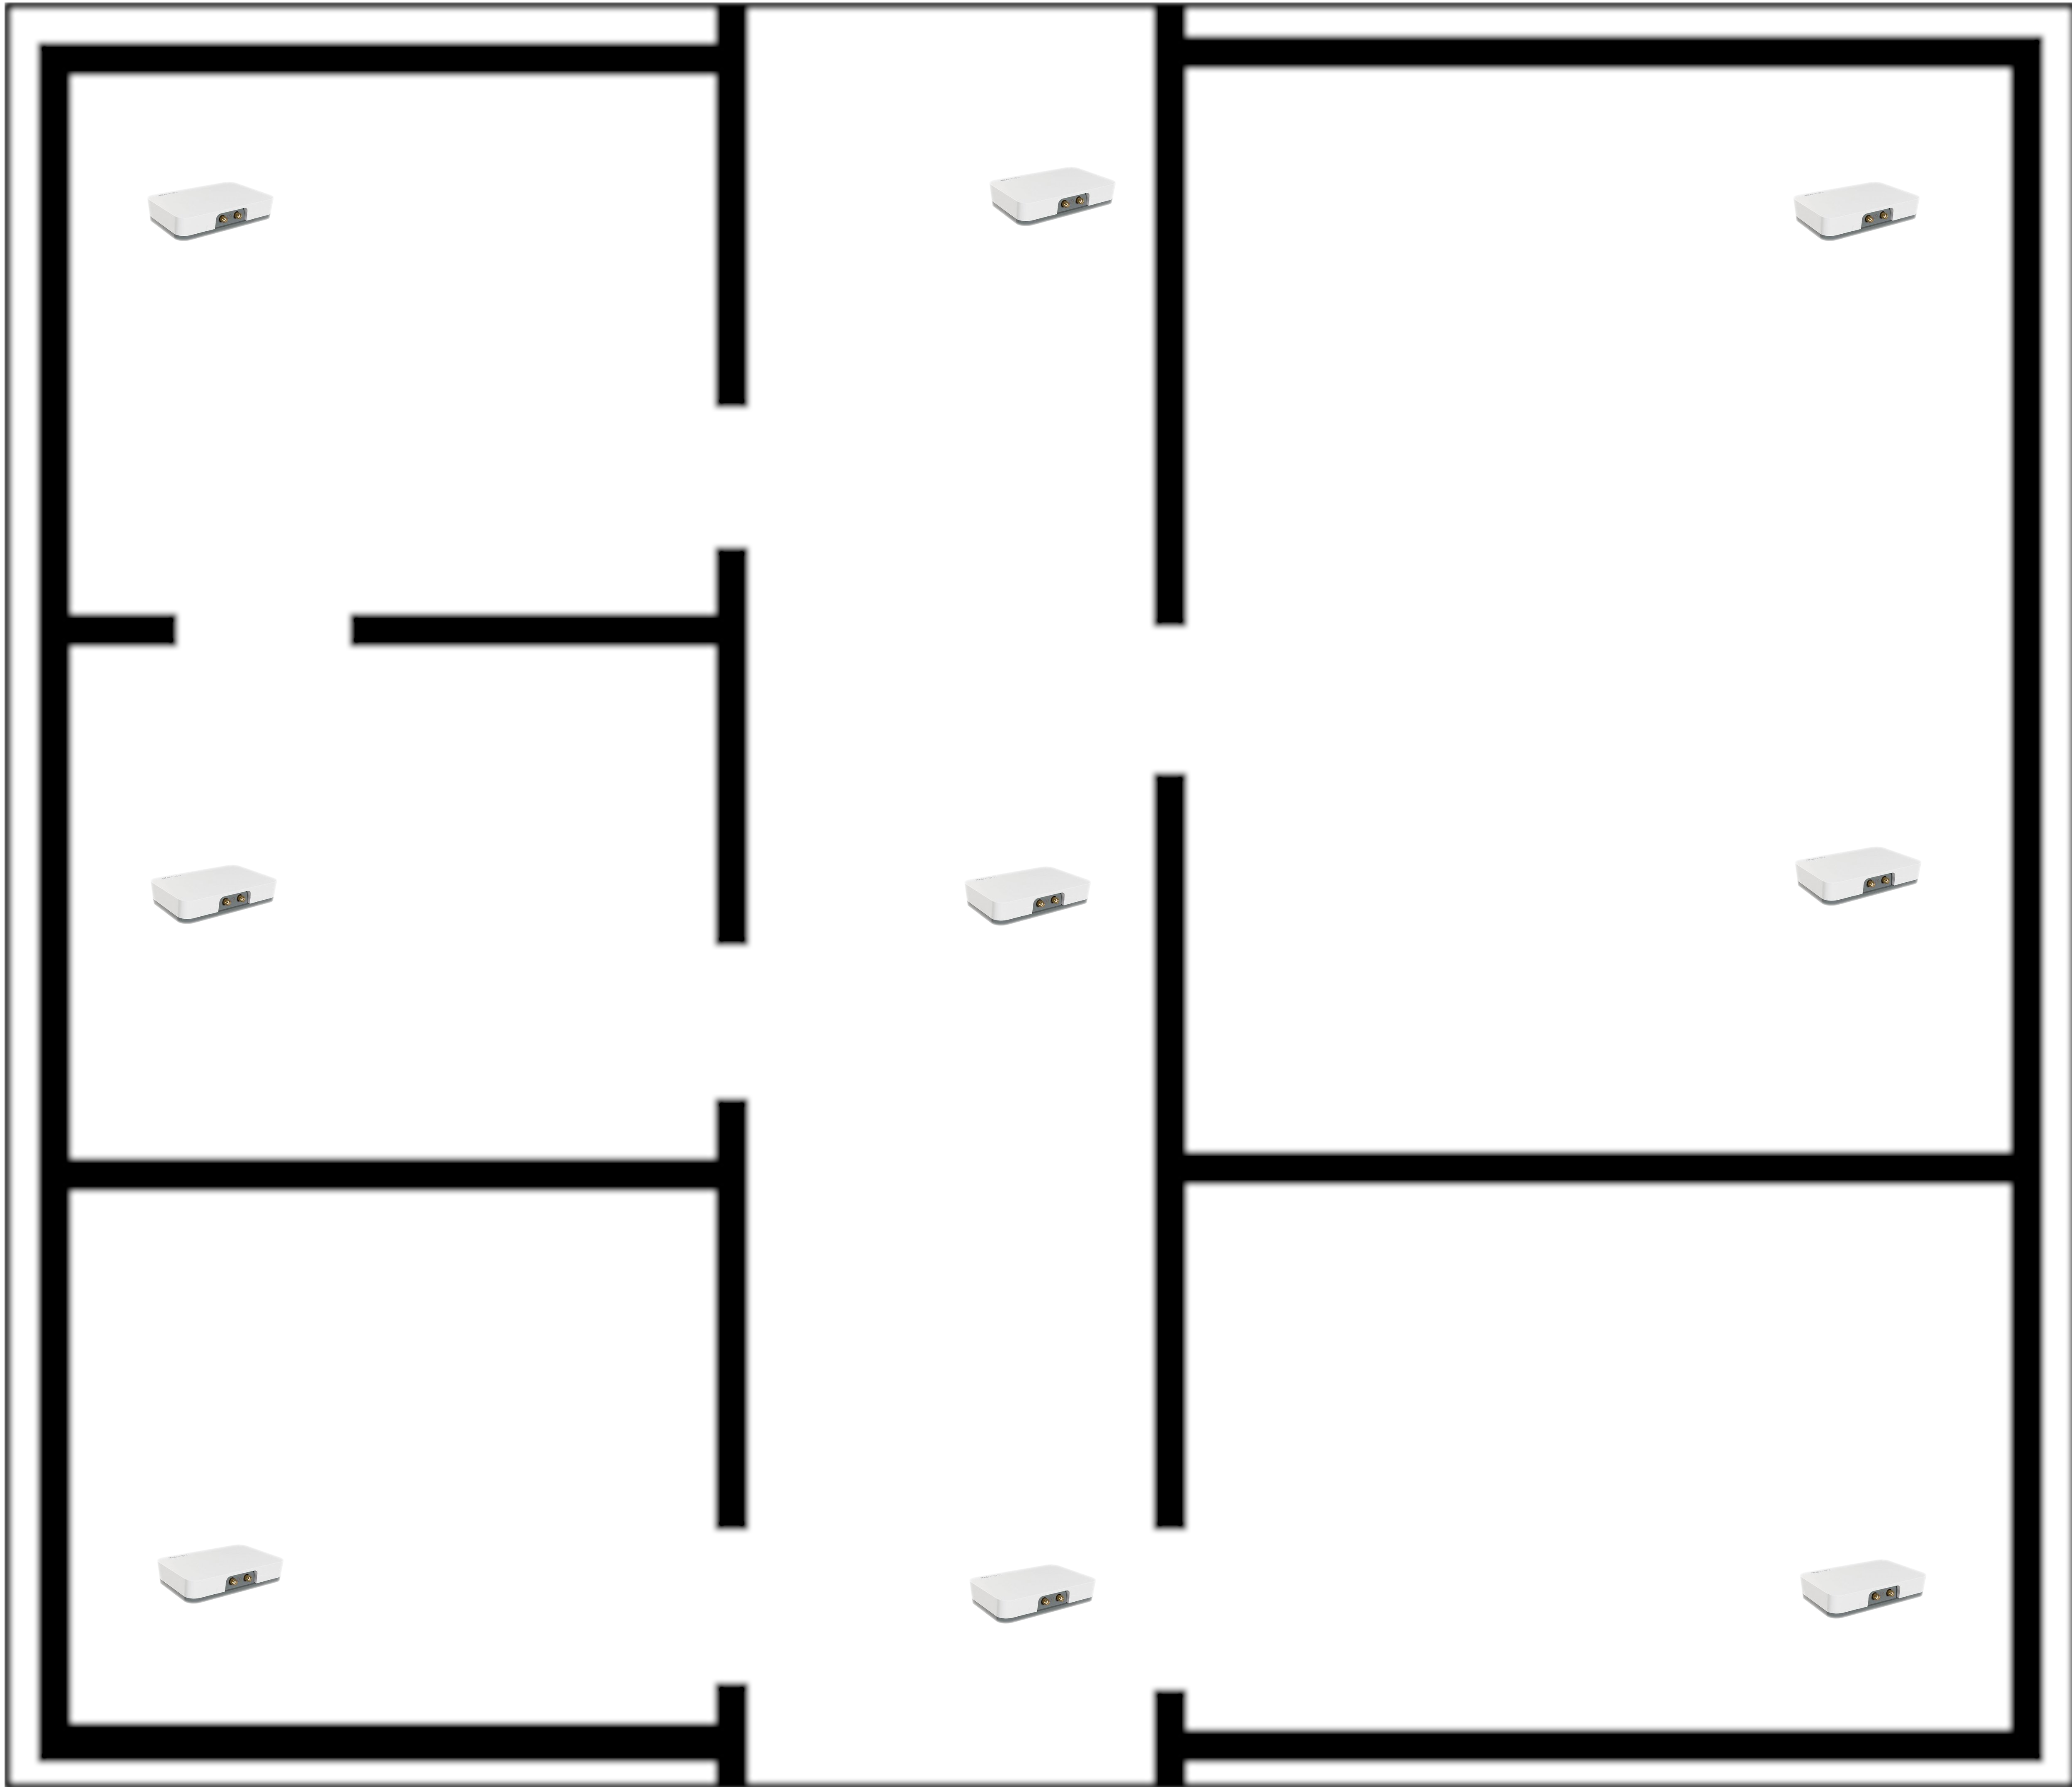
\includegraphics[width=\linewidth]{ble_statisch_3}
\end{minipage}


\subsection{Dynamisch}

\subsubsection{1 beacon per locatie, midden van kamer}
%TODO

\subsubsection{1 beacon per locatie, aan deur}
%TODO

\subsubsection{< 1 beacon per locatie}
%TODO

\subsubsection{> 1 beacon per locatie}
%TODO

\subsubsection{beacons op intervallen in de gang}
%TODO
%\input{...}
%...

%%=============================================================================
%% Conclusie
%%=============================================================================

\chapter{Conclusie}
\label{ch:conclusie}
\section{Informatiebundeling}
\label{sec:con-inf}
Voordat een algemene conclusie getrokken kan worden, is het interessant alle relevante informatie op een rijtje te plaatsen. Hieronder volgt een opsomming van alle onderzochte opstellingen, waarbij voor elk hun toepassingsgebied wordt bijgevoegd, alsook de eventuele \textcolor{ForestGreen}{voor-} en \textcolor{RedOrange}{nadelen}. Al deze informatie is reeds beschikbaar in het corpus en voornamelijk de deelconclusies in hoofdstuk~\ref{ch:testen}. De informatie voor de algemene voor- en nadelen wordt gehaald uit hoofdstuk~\ref{ch:opstellingen}. Deze gelden voor elke opstelling in de specifieke technologie.

Ook wordt er een benadering gegeven voor de kostprijs, de informatie voor deze berekening is reeds beschikbaar in hoofdstuk~\ref{ch:methodologie}. Deze kostprijs \(K\) wordt uitgedrukt als \(K = f(l, a)\) met \(l\) het aantal locaties en \(a\) het aantal assets. Dit zijn de 2 voornaamste schaalfactoren voor de kosten.

Het doel van deze sectie is een gestructureerde weergave van de meest interessante informatie te geven, als basis voor het nemen van de feitelijke eindconclusie.

\subsection{RFID Algemeen}
\label{sec:con-ant-RFID}
\paragraph{Voor- en nadelen}
\begin{itemize}
	\color{ForestGreen}
	\item Goedkope tags
	\item Tags vereisen geen/minimaal onderhoud
	\color{RedOrange}
	\item Dure uitrolkosten
	\item Tags enkel detecteerbaar in RFID doorgang
	\item Tagoriëntatie in de RFID doorgang is belangrijk
\end{itemize}

\subsection{BLE Algemeen}
\label{sec:con-ant-BLE}
\paragraph{Voor- en nadelen}
\begin{itemize}
	\color{ForestGreen}
	\item Beacons steeds detecteerbaar
	\item Goedkope uitrolkosten
	\item Tagoriëntatie verwaarloosbaar
	\color{RedOrange}
	\item Beacons vereisen onderhoud
	\item Relatief dure beacons
	\item Grote variatie op RSSI waarden
\end{itemize}

\subsection{Static RFID: 1 antenne aan deurlijst}
Bruikbaar bij afgesloten ruimtes met (smalle) toegangen als locatie.
\paragraph{Voor- en nadelen}
\begin{itemize}
\color{ForestGreen}
\item Goedkoopste/minimale RFID optie
\color{RedOrange}
\item Geen richtingsdetectie
\item Enkel te gebruiken in deurdoorgang
\end{itemize}
\paragraph{Kostprijs}
\(K = 1400 \cdot l + 0.01 \cdot a\)

\emph{De kostprijs per locatie kan verlaagd worden door meerdere antennes op 1 transceiver aan te sluiten, als de in-/uitgangen van deze locaties dicht genoeg bij elkaar liggen}

\subsection{Static RFID: 2 antennes aan deurlijst}
Bruikbaar bij afgesloten ruimtes met (smalle) toegangen als locatie.
\paragraph{Voor- en nadelen}
\begin{itemize}
	\color{ForestGreen}
	\item Richtingsdetectie
	\color{RedOrange}
	\item Past moeilijker in deurlijst door breedte 2 antennes + eventuele tussenafstand bij bredere doorgang.
	\item Enkel te gebruiken in deurdoorgang
\end{itemize}
\paragraph{Kostprijs}
\(K = 1450 \cdot l + 0.01 \cdot a\)

\emph{De kostprijs per locatie kan verlaagd worden door 2 antenneparen op 1 4-port transceiver aan te sluiten, als de in-/uitgangen van deze locaties dicht genoeg bij elkaar liggen}

\subsection{Static RFID: 1 antenne tegenover deur}
Bruikbaar bij afgesloten ruimtes met een (korte) gang als toegang, als locatie.
\paragraph{Voor- en nadelen}
\begin{itemize}
	\color{ForestGreen}
	\item Richtingsdetectie
	\item Slechts 1 antenne
	\color{RedOrange}
	\item Vereist langere gang dan enkel deurdoorgang voor goede werking
\end{itemize}
\paragraph{Kostprijs}
\(K = 1400 \cdot l + 0.01 \cdot a\)

\emph{De kostprijs per locatie kan verlaagd worden door meerdere antennes op 1 transceiver aan te sluiten, als de in-/uitgangen van deze locaties dicht genoeg bij elkaar liggen}

\subsection{Dynamic RFID: 1 tag aan deurlijst}
Bruikbaar bij afgesloten ruimtes met (smalle) toegangen, als locatie.
\paragraph{Voor- en nadelen}
\begin{itemize}
	\color{ForestGreen}
	\item Goedkoop door slechts 1 reader
	\color{RedOrange}
	\item Niet noodzakelijk detectie van \emph{alle} aanwezige assets.
\end{itemize}
\paragraph{Kostprijs}
\(K = 1400 + 0.01 \cdot (l + a)\)

\subsection{Static BLE: 1 gateway per locatie}
Bruikbaar bij alle reële locaties gescheiden door muren.
\paragraph{Voor- en nadelen}
\begin{itemize}
	\color{ForestGreen}
	\item Goedkoop
	\item Eenvoudig
	\color{RedOrange}
	\item Niet goed bruikbaar bij meerdere locaties in open ruimte.
\end{itemize}
\paragraph{Kostprijs}
\(K = 100 \cdot l + 10 \cdot a\)

\subsection{Static BLE: meerdere gateways per locatie}
Overal bruikbaar, bij reële locaties gescheiden door muren vereenvoudiging mogelijk.
\paragraph{Voor- en nadelen}
\begin{itemize}
	\color{ForestGreen}
	\item Goede werking bij meerdere locaties in open ruimte.
	\color{RedOrange}
	\item Hogere hardwarekost
	\item Kan worden vereenvoudigd
\end{itemize}
\paragraph{Kostprijs}
\(K = 400 \cdot l + 10 \cdot a\)

\emph{Veronderstelling van omringing door 4 gateways, meer of minder is mogelijk.}

\subsection{Static BLE: gateways in rasteropstelling}
Nergens bruikbaar
\paragraph{Voor- en nadelen}
\begin{itemize}
	\color{ForestGreen}
	\item Lagere hardwarekost door geen 1:1 relatie tussen locatiebeacons en locaties
	\item Locatiedefinities veranderbaar zonder hardware aanpassingen
	\color{RedOrange}
	\item Werkt niet
	\item Meer overhead door nood aan locatiedefiniëring
\end{itemize}
\paragraph{Kostprijs}
\(K = \ll100 \cdot l + 10 \cdot a\)

\emph{Er kan ook meer dan 1 gateway per locatie in een raster staan, in dat geval zijn er echter goedkopere opstellingen mogelijk}

\subsection{Dynamic BLE: 1 locatiebeacon per locatie, midden van locatie}
Overal bruikbaar
\paragraph{Voor- en nadelen}
\begin{itemize}
	\color{ForestGreen}
	\item Lage hardwarekost
	\item Werkt overal
	\color{RedOrange}
	\item Geen real-time detectie
	\item Hoog batterijgebruik
\end{itemize}
\paragraph{Kostprijs}
\(K = 100 + 10 \cdot (l + a)\)

\subsection{Dynamic BLE: 1 locatiebeacon per locatie, aan deur}
Overal bruikbaar
\paragraph{Voor- en nadelen}
\begin{itemize}
	\color{ForestGreen}
	\item Lage hardwarekost
	\item Werkt overal
	\item Nauwkeurigere detectie dan met beacon in midden van kamer
	\color{RedOrange}
	\item Geen real-time detectie
	\item Meer overhead als deur met beacon niet in midden van kamer zit
	\item Hoog batterijgebruik
\end{itemize}
\paragraph{Kostprijs}
\(K = 100 + 10 \cdot (l + a)\)

\subsection{Dynamic BLE: meerdere locatiebeacons per locatie}
Overal bruikbaar, bij reële locaties gescheiden door muren vereenvoudiging mogelijk.
\paragraph{Voor- en nadelen}
\begin{itemize}
	\color{ForestGreen}
	\item Lage hardwarekost
	\item Werkt overal
	\color{RedOrange}
	\item Geen real-time detectie
	\item Kan worden vereenvoudigd
	\item Hoog batterijgebruik
\end{itemize}
\paragraph{Kostprijs}
\(K = 100 + 10 \cdot (l + a)\)

\subsection{Dynamic BLE: locatiebeacons in rasteropstelling}
Nergens bruikbaar
\paragraph{Voor- en nadelen}
\begin{itemize}
	\color{ForestGreen}
	\item Nog lagere hardwarekost door geen 1:1 relatie tussen locatiebeacons en locaties
	\item Locatiedefinities veranderbaar zonder hardware aanpassingen
	\color{RedOrange}
	\item Werkt niet
	\item Meer overhead door nood aan locatiedefiniëring
	\item Hoog batterijgebruik
\end{itemize}
\paragraph{Kostprijs}
\(K = 100 + 10 \cdot (\ll l + a)\)

\emph{Er kan ook meer dan 1 locatiebeacon per locatie in een raster staan, in dat geval zijn er echter goedkopere opstellingen mogelijk}

\subsection{Dynamic BLE: locatiebeacons op intervallen in de gang}
Overal bruikbaar
\paragraph{Voor- en nadelen}
\begin{itemize}
	\color{ForestGreen}
	\item Nog lagere hardwarekost door geen 1:1 relatie tussen locatiebeacons en locaties
	\item Locatiedefinities veranderbaar zonder hardware aanpassingen
	\color{RedOrange}
	\item Geen real-time detectie
	\item Meer overhead door nood aan locatiedefiniëring
	\item Hoog batterijgebruik
\end{itemize}
\paragraph{Kostprijs}
\(K = 100 + 10 \cdot (\ll l + a)\)

\emph{Er kan ook meer dan 1 locatiebeacon per locatie in de gangen hangen, in dat geval zijn er echter goedkopere opstellingen mogelijk}

\section{Een antwoord op de onderzoeksvraag}
\label{sec:con-ant}
Na opsomming van de belangrijkste conclusies van alle onderzochte opstellingen in sectie~\ref{sec:con-inf}, is de tijd gekomen om een antwoord te formuleren op de onderzoeksvraag van dit onderzoek. Deze vraag luid als volgt \footnote{Zie Sectie~\ref{sec:onderzoeksvraag} op pagina~\pageref{sec:onderzoeksvraag}}.:
\begin{center}
	\textbf{Welke hardwareopstelling, bestaande uit RFID of BLE componenten, is optimaal voor de plaats- en verplaatsingsbepaling van een voorwerp binnen een gebouw.}
\end{center}

Om een antwoord te geven op deze onderzoeksvraag moet een vergelijking gemaakt worden tussen alle opstellingen. Een goed begin hiervoor is bij de gebruikte technologie.

\paragraph{RFID vs BLE}
Zoals aangehaald in secties~\ref{sec:con-ant-RFID} en~\ref{sec:con-ant-BLE} heeft elk van deze technologieën zijn voor- en nadelen. Echter is hier de vraag welke van deze voor- en nadelen het meeste doorweegt voor een goede en bruikbare lokalisatieopstelling. 
Het fundamentele voordeel van BLE op dit vlak is nog steeds dat de getagde assets steeds zichtbaar zijn voor het systeem, en er altijd zeker is geweten of het asset aanwezig is, en waar, dit is niet het geval bij RFID. 

Verder heeft BLE een voordeel door de lagere uitrolkosten van een systeem, wat de aanschafdrempel voor heel wat bedrijven, zeker deze met een kleiner budget, kan verlagen. De opschalingskosten, met name deze om meer assets te taggen, zijn hoger dan bij RFID, maar dit is voor toepassingen met een beperkt aantal assets niet zo'n probleem. Ook kan dit geleidelijk aan gebeuren samen met de groei van een bedrijf. Bijvoorbeeld een initiële investering van €5000 voor een systeem en elk jaar €2000 voor nieuwe beacons is realistisch, maar een uitrolkost van €50000 voor een RFID systeem, hoe klein de kost daarna ook mag zijn is veel onaantrekkelijker. Slechts als de kosten van de beacons in de buurt komt van de initiële kost van een RFID opstelling kan er een degelijke vergelijking gemaakt worden. Deze argumenten in acht nemend is het duidelijk dat BLE met oog op de onderzoeksvraag voor dit onderzoek de bovenhand heeft. De beste opstelling zal hierdoor komen uit de 8 BLE opstellingen.

\paragraph{Statisch vs Dynamisch}
Het volgende bestaande onderscheid is deze tussen de statische en dynamische opstellingen. Hier is het zo dat bij beide categorieën opstellingen bestaan die een perfecte lokalisatie bekomen van de assets. Hier bestaat een gelijkstand. Echter is dit niet het enige criteria in de onderzoeksvraag. Ook de detectie van een verplaatsing is vereist, en op dit vlak is er een falen van de dynamische opstellingen. Dit voornamelijk door hun fundamentele niet real-time aard. Bij dynamische opstellingen worden de assets enkel gedetecteerd als de gateway rondgaat in het gebouw. Op dat moment kan een asset al lang verplaatst zijn en is deze niet, of in het beste geval later gedetecteerd. In tegenstelling tot een statische opstelling, waarbij deze verplaatsing meteen wordt gedetecteerd van zodra de gemeten RSSI waarden zo veranderen dat deze bij een andere locatie wordt gecategoriseerd. Statische opstellingen hebben een betere, of op zijn minst snellere detectie, van een verplaatsing. 

Verder is het wel zo dat de kostprijs van een statische opstelling hoger licht dan deze van een dynamische. Echter is dit verschil niet zo uitgesproken, en nog steeds draagbaar (€100 voor een gateway is niet zo veel, en zeker niet zo veel meer dan de €10 voor een beacon). Verder is er qua kostprijs ook de onderhoudskost te bekijken. Voor een dynamische opstelling moeten de beacons op elk moment zeer snel staan ingesteld, wat de batterijduur veel verkort en waardoor er sneller nieuwe batterijen, of nieuwe beacons als de batterij onvervangbaar is, nodig zijn. Bij statische opstellingen kunnen de beacons veel trager ingesteld staan en nog steeds een acceptabele lokalisatie geven, met langere batterijduur tot gevolg. Daarom zal de beste opstelling een van de drie statische opstellingen zijn.

\paragraph{De keuze}
Na vorige schiftingen blijven er nog 3 opstellingen over. Als eerste is het duidelijk dat de rasteropstelling niet de beste is, aangezien deze zeer slechte resultaten leverde. Verder is het, qua toepassingsgebied, duidelijk dat de opstelling met meerdere gateways per locatie de beste is uit de 2 overgebleven, aangezien deze werkt in een open ruimte en de opstelling met 1 gateway niet. Echter is het zo dat bij een situatie waarbij elke locatie omringt is door een muur, deze kan vereenvoudigd worden naar de opstelling met 1 gateway per locatie. Een combinatie van deze 2 opstellingen lijkt hierdoor het meest toegewezen om het probleem aangekaart in de onderzoeksvraag op te lossen.

\paragraph{Het effectieve antwoord}
Het antwoord op de onderzoeksvraag luid als volgt:
\begin{center}
	\textbf{Een combinatie van 2 statische BLE opstellingen, nl. 1 gateway per locatie voor ommuurde locaties, en meerdere gateways per locatie voor meerdere locaties in een open ruimte, is optimaal voor de plaats- en verplaatsingsbepaling van een voorwerp binnen een gebouw.}
\end{center}

\section{Nawoord}
Het is ook duidelijk dat, hoewel dit de beste optie is als antwoord op de onderzoeksvraag zoals ze gesteld is, het merendeel van de andere opstellingen ook hun toepassingsgebied hebben. 

Statische RFID opstellingen, hoewel hier achterwege gelaten voornamelijk door de hoge initiële kost, heeft toepassingen bij zeer hoge volumes assets. Dit is ook niet verrassend aangezien toepassingen van deze opstellingen de voornaamste bezigheid is van Aucxis, en zeker voor de toevoeging van BLE aan hun palmares. 

Dynamische BLE opstellingen hebben ook uitermate goed gepresteerd, en hier zit zeker potentieel in. Het leent zich meer voor concepten zoals inventarisatie, waarbij de eis kan zijn dat er 1x per dag een update van locaties moet zijn en de mobiele gateway bv. aan de kar van de poetsvrouw kan hangen. Echter is het niet geschikt voor (real-time) verplaatsingsdetectie zoals de eis was voor dit onderzoek.

\section{Verder onderzoek}
Dit onderzoek is voornamelijk bedoeld als verkennend, het verkennen van veel verschillende soorten opstellingen zonder al te diep erop in te gaan. Er is nu een antwoord uit de bus gekomen, maar dit is in essentie de optie die het meeste kans maakt om optimaal te zijn. Hierbij is verder onderzoek nodig naar de invloed van verschillende factoren die tijdens dit onderzoek constant zijn genomen. Dit zijn voornamelijk de invloed van de grootte van de locaties (opschalen van de testopstelling) en de invloed van de zendsterkte van de beacons. Maar verder ook meer specifieke variabelen zoals de soort gateway en beacons, de inhoud van de locaties (qua meubels en eventueel reflecterende materialen), het soort muren en deuren en zo veel andere beïnvloedende factoren. Het spreekt voor zich dat een onderzoek naar al deze factoren een onderzoek is van dezelfde grootteorde als deze, en dit niet meer bij de scope van dit onderzoek hoort.

Verder zijn tijdens dit onderzoek de opstellingen in een raster met trilateratie gefaald door de limitatie van het zeer onjuiste omrekening van RSSI waardes naar afstand. Echter is dit niet de enige mogelijkheid om uit deze data een locatie te bepalen, en hoogstwaarschijnlijk kan er, na enig onderzoek, een algoritme bedacht worden die wel acceptabele resultaten geeft. Dit lag echter ook buiten de scope van dit onderzoek.

%%=============================================================================
%% Bijlagen
%%=============================================================================

\appendix
\renewcommand{\chaptername}{Appendix}

%%---------- Onderzoeksvoorstel -----------------------------------------------

\chapter{Onderzoeksvoorstel}

Het onderwerp van deze bachelorproef is gebaseerd op een onderzoeksvoorstel dat vooraf werd beoordeeld door de promotor. Dat voorstel is opgenomen in deze bijlage.

%%---------- Andere bijlagen --------------------------------------------------
% TODO: Voeg hier eventuele andere bijlagen toe
%\input{...}

%%---------- Referentielijst --------------------------------------------------
\chapter{Bibliografie}
\printbibliography[heading=bibintoc]
\end{document}
